% Options for packages loaded elsewhere
\PassOptionsToPackage{unicode}{hyperref}
\PassOptionsToPackage{hyphens}{url}
\PassOptionsToPackage{dvipsnames,svgnames,x11names}{xcolor}
%
\documentclass[
  letterpaper,
  DIV=11,
  numbers=noendperiod]{scrartcl}

\usepackage{amsmath,amssymb}
\usepackage{iftex}
\ifPDFTeX
  \usepackage[T1]{fontenc}
  \usepackage[utf8]{inputenc}
  \usepackage{textcomp} % provide euro and other symbols
\else % if luatex or xetex
  \usepackage{unicode-math}
  \defaultfontfeatures{Scale=MatchLowercase}
  \defaultfontfeatures[\rmfamily]{Ligatures=TeX,Scale=1}
\fi
\usepackage{lmodern}
\ifPDFTeX\else  
    % xetex/luatex font selection
\fi
% Use upquote if available, for straight quotes in verbatim environments
\IfFileExists{upquote.sty}{\usepackage{upquote}}{}
\IfFileExists{microtype.sty}{% use microtype if available
  \usepackage[]{microtype}
  \UseMicrotypeSet[protrusion]{basicmath} % disable protrusion for tt fonts
}{}
\makeatletter
\@ifundefined{KOMAClassName}{% if non-KOMA class
  \IfFileExists{parskip.sty}{%
    \usepackage{parskip}
  }{% else
    \setlength{\parindent}{0pt}
    \setlength{\parskip}{6pt plus 2pt minus 1pt}}
}{% if KOMA class
  \KOMAoptions{parskip=half}}
\makeatother
\usepackage{xcolor}
\setlength{\emergencystretch}{3em} % prevent overfull lines
\setcounter{secnumdepth}{-\maxdimen} % remove section numbering
% Make \paragraph and \subparagraph free-standing
\makeatletter
\ifx\paragraph\undefined\else
  \let\oldparagraph\paragraph
  \renewcommand{\paragraph}{
    \@ifstar
      \xxxParagraphStar
      \xxxParagraphNoStar
  }
  \newcommand{\xxxParagraphStar}[1]{\oldparagraph*{#1}\mbox{}}
  \newcommand{\xxxParagraphNoStar}[1]{\oldparagraph{#1}\mbox{}}
\fi
\ifx\subparagraph\undefined\else
  \let\oldsubparagraph\subparagraph
  \renewcommand{\subparagraph}{
    \@ifstar
      \xxxSubParagraphStar
      \xxxSubParagraphNoStar
  }
  \newcommand{\xxxSubParagraphStar}[1]{\oldsubparagraph*{#1}\mbox{}}
  \newcommand{\xxxSubParagraphNoStar}[1]{\oldsubparagraph{#1}\mbox{}}
\fi
\makeatother

\usepackage{color}
\usepackage{fancyvrb}
\newcommand{\VerbBar}{|}
\newcommand{\VERB}{\Verb[commandchars=\\\{\}]}
\DefineVerbatimEnvironment{Highlighting}{Verbatim}{commandchars=\\\{\}}
% Add ',fontsize=\small' for more characters per line
\usepackage{framed}
\definecolor{shadecolor}{RGB}{241,243,245}
\newenvironment{Shaded}{\begin{snugshade}}{\end{snugshade}}
\newcommand{\AlertTok}[1]{\textcolor[rgb]{0.68,0.00,0.00}{#1}}
\newcommand{\AnnotationTok}[1]{\textcolor[rgb]{0.37,0.37,0.37}{#1}}
\newcommand{\AttributeTok}[1]{\textcolor[rgb]{0.40,0.45,0.13}{#1}}
\newcommand{\BaseNTok}[1]{\textcolor[rgb]{0.68,0.00,0.00}{#1}}
\newcommand{\BuiltInTok}[1]{\textcolor[rgb]{0.00,0.23,0.31}{#1}}
\newcommand{\CharTok}[1]{\textcolor[rgb]{0.13,0.47,0.30}{#1}}
\newcommand{\CommentTok}[1]{\textcolor[rgb]{0.37,0.37,0.37}{#1}}
\newcommand{\CommentVarTok}[1]{\textcolor[rgb]{0.37,0.37,0.37}{\textit{#1}}}
\newcommand{\ConstantTok}[1]{\textcolor[rgb]{0.56,0.35,0.01}{#1}}
\newcommand{\ControlFlowTok}[1]{\textcolor[rgb]{0.00,0.23,0.31}{\textbf{#1}}}
\newcommand{\DataTypeTok}[1]{\textcolor[rgb]{0.68,0.00,0.00}{#1}}
\newcommand{\DecValTok}[1]{\textcolor[rgb]{0.68,0.00,0.00}{#1}}
\newcommand{\DocumentationTok}[1]{\textcolor[rgb]{0.37,0.37,0.37}{\textit{#1}}}
\newcommand{\ErrorTok}[1]{\textcolor[rgb]{0.68,0.00,0.00}{#1}}
\newcommand{\ExtensionTok}[1]{\textcolor[rgb]{0.00,0.23,0.31}{#1}}
\newcommand{\FloatTok}[1]{\textcolor[rgb]{0.68,0.00,0.00}{#1}}
\newcommand{\FunctionTok}[1]{\textcolor[rgb]{0.28,0.35,0.67}{#1}}
\newcommand{\ImportTok}[1]{\textcolor[rgb]{0.00,0.46,0.62}{#1}}
\newcommand{\InformationTok}[1]{\textcolor[rgb]{0.37,0.37,0.37}{#1}}
\newcommand{\KeywordTok}[1]{\textcolor[rgb]{0.00,0.23,0.31}{\textbf{#1}}}
\newcommand{\NormalTok}[1]{\textcolor[rgb]{0.00,0.23,0.31}{#1}}
\newcommand{\OperatorTok}[1]{\textcolor[rgb]{0.37,0.37,0.37}{#1}}
\newcommand{\OtherTok}[1]{\textcolor[rgb]{0.00,0.23,0.31}{#1}}
\newcommand{\PreprocessorTok}[1]{\textcolor[rgb]{0.68,0.00,0.00}{#1}}
\newcommand{\RegionMarkerTok}[1]{\textcolor[rgb]{0.00,0.23,0.31}{#1}}
\newcommand{\SpecialCharTok}[1]{\textcolor[rgb]{0.37,0.37,0.37}{#1}}
\newcommand{\SpecialStringTok}[1]{\textcolor[rgb]{0.13,0.47,0.30}{#1}}
\newcommand{\StringTok}[1]{\textcolor[rgb]{0.13,0.47,0.30}{#1}}
\newcommand{\VariableTok}[1]{\textcolor[rgb]{0.07,0.07,0.07}{#1}}
\newcommand{\VerbatimStringTok}[1]{\textcolor[rgb]{0.13,0.47,0.30}{#1}}
\newcommand{\WarningTok}[1]{\textcolor[rgb]{0.37,0.37,0.37}{\textit{#1}}}

\providecommand{\tightlist}{%
  \setlength{\itemsep}{0pt}\setlength{\parskip}{0pt}}\usepackage{longtable,booktabs,array}
\usepackage{calc} % for calculating minipage widths
% Correct order of tables after \paragraph or \subparagraph
\usepackage{etoolbox}
\makeatletter
\patchcmd\longtable{\par}{\if@noskipsec\mbox{}\fi\par}{}{}
\makeatother
% Allow footnotes in longtable head/foot
\IfFileExists{footnotehyper.sty}{\usepackage{footnotehyper}}{\usepackage{footnote}}
\makesavenoteenv{longtable}
\usepackage{graphicx}
\makeatletter
\def\maxwidth{\ifdim\Gin@nat@width>\linewidth\linewidth\else\Gin@nat@width\fi}
\def\maxheight{\ifdim\Gin@nat@height>\textheight\textheight\else\Gin@nat@height\fi}
\makeatother
% Scale images if necessary, so that they will not overflow the page
% margins by default, and it is still possible to overwrite the defaults
% using explicit options in \includegraphics[width, height, ...]{}
\setkeys{Gin}{width=\maxwidth,height=\maxheight,keepaspectratio}
% Set default figure placement to htbp
\makeatletter
\def\fps@figure{htbp}
\makeatother

\usepackage{booktabs}
\usepackage{caption}
\usepackage{longtable}
\usepackage{colortbl}
\usepackage{array}
\usepackage{anyfontsize}
\usepackage{multirow}
\KOMAoption{captions}{tableheading}
\makeatletter
\@ifpackageloaded{caption}{}{\usepackage{caption}}
\AtBeginDocument{%
\ifdefined\contentsname
  \renewcommand*\contentsname{Table of contents}
\else
  \newcommand\contentsname{Table of contents}
\fi
\ifdefined\listfigurename
  \renewcommand*\listfigurename{List of Figures}
\else
  \newcommand\listfigurename{List of Figures}
\fi
\ifdefined\listtablename
  \renewcommand*\listtablename{List of Tables}
\else
  \newcommand\listtablename{List of Tables}
\fi
\ifdefined\figurename
  \renewcommand*\figurename{Figure}
\else
  \newcommand\figurename{Figure}
\fi
\ifdefined\tablename
  \renewcommand*\tablename{Table}
\else
  \newcommand\tablename{Table}
\fi
}
\@ifpackageloaded{float}{}{\usepackage{float}}
\floatstyle{ruled}
\@ifundefined{c@chapter}{\newfloat{codelisting}{h}{lop}}{\newfloat{codelisting}{h}{lop}[chapter]}
\floatname{codelisting}{Listing}
\newcommand*\listoflistings{\listof{codelisting}{List of Listings}}
\makeatother
\makeatletter
\makeatother
\makeatletter
\@ifpackageloaded{caption}{}{\usepackage{caption}}
\@ifpackageloaded{subcaption}{}{\usepackage{subcaption}}
\makeatother

\ifLuaTeX
  \usepackage{selnolig}  % disable illegal ligatures
\fi
\usepackage{bookmark}

\IfFileExists{xurl.sty}{\usepackage{xurl}}{} % add URL line breaks if available
\urlstyle{same} % disable monospaced font for URLs
\hypersetup{
  pdftitle={Simulation},
  colorlinks=true,
  linkcolor={blue},
  filecolor={Maroon},
  citecolor={Blue},
  urlcolor={Blue},
  pdfcreator={LaTeX via pandoc}}


\title{Simulation}
\author{}
\date{}

\begin{document}
\maketitle


\section{1. Dataset}\label{dataset}

Vignettes only (Yunnan 2017, NCD 2018, Three Province2015)

\section{2. Data Analysis}\label{data-analysis}

\subsection{2.0 Import Data}\label{import-data}

\begin{Shaded}
\begin{Highlighting}[]
\FunctionTok{install.packages}\NormalTok{(}\StringTok{"Hmisc"}\NormalTok{)}
\end{Highlighting}
\end{Shaded}

\begin{verbatim}
Installing Hmisc [5.2-2] ...
    OK [linked cache]
\end{verbatim}

\begin{Shaded}
\begin{Highlighting}[]
\NormalTok{knitr}\SpecialCharTok{::}\NormalTok{opts\_chunk}\SpecialCharTok{$}\FunctionTok{set}\NormalTok{(}\AttributeTok{echo =} \ConstantTok{TRUE}\NormalTok{, }\AttributeTok{message =} \ConstantTok{FALSE}\NormalTok{, }\AttributeTok{warning =} \ConstantTok{FALSE}\NormalTok{)}

\FunctionTok{library}\NormalTok{(haven)}
\NormalTok{visit\_data }\OtherTok{\textless{}{-}} \FunctionTok{read\_dta}\NormalTok{(}\StringTok{"data{-}raw/vig\_clean\_all.dta"}\NormalTok{)}
\end{Highlighting}
\end{Shaded}

\subsection{2.1 Basic Information
Tables}\label{basic-information-tables}

\subsubsection{2.1.1 Table 1 Summary of correct/partially
diagnosis/checklist (N=2564: Angina = 980, Diarrhea = 627, TB = 319,
Hypertension =
638)}\label{table-1-summary-of-correctpartially-diagnosischecklist-n2564-angina-980-diarrhea-627-tb-319-hypertension-638}

\begin{Shaded}
\begin{Highlighting}[]
\CommentTok{\# descriptive analysis}

\FunctionTok{library}\NormalTok{(gtsummary)}
\FunctionTok{library}\NormalTok{(}\StringTok{"dplyr"}\NormalTok{)}

\CommentTok{\# create new variables needed for the analysis}
\NormalTok{visit\_data}\SpecialCharTok{$}\NormalTok{disease\_num }\OtherTok{\textless{}{-}} \FunctionTok{factor}\NormalTok{(visit\_data}\SpecialCharTok{$}\NormalTok{disease\_num,}
                                          \AttributeTok{levels =} \FunctionTok{c}\NormalTok{(}\DecValTok{1}\NormalTok{, }\DecValTok{2}\NormalTok{, }\DecValTok{3}\NormalTok{, }\DecValTok{4}\NormalTok{),}
                                          \AttributeTok{labels =} \FunctionTok{c}\NormalTok{(}\StringTok{"Angina"}\NormalTok{, }\StringTok{"Diarrhea"}\NormalTok{, }\StringTok{"TB"}\NormalTok{, }\StringTok{"Hypertension"}\NormalTok{))}

\CommentTok{\# select the variables}
\NormalTok{visit\_vars }\OtherTok{\textless{}{-}}\NormalTok{ visit\_data }\SpecialCharTok{\%\textgreater{}\%}
                \FunctionTok{select}\NormalTok{(corrdiag, pcorrdiag, wrongdiag, nrq, arq )}
\NormalTok{visit\_var }\OtherTok{\textless{}{-}}\NormalTok{ visit\_data }\SpecialCharTok{\%\textgreater{}\%}
                \FunctionTok{select}\NormalTok{(corrdiag, pcorrdiag, wrongdiag, nrq, arq, disease\_num )}

\CommentTok{\# All sample}
\NormalTok{all\_visit }\OtherTok{\textless{}{-}}\NormalTok{ visit\_vars }\SpecialCharTok{\%\textgreater{}\%}
                  \FunctionTok{tbl\_summary}\NormalTok{(}
                    \AttributeTok{missing =} \StringTok{"no"}\NormalTok{,}
                    \AttributeTok{type =} \FunctionTok{list}\NormalTok{(}
\NormalTok{                                corrdiag }\SpecialCharTok{\textasciitilde{}} \StringTok{"dichotomous"}\NormalTok{,}
\NormalTok{                                pcorrdiag }\SpecialCharTok{\textasciitilde{}} \StringTok{"dichotomous"}\NormalTok{,}
\NormalTok{                                wrongdiag }\SpecialCharTok{\textasciitilde{}} \StringTok{"dichotomous"}\NormalTok{,}
\NormalTok{                                nrq }\SpecialCharTok{\textasciitilde{}} \StringTok{"continuous"}\NormalTok{,}
\NormalTok{                                arq }\SpecialCharTok{\textasciitilde{}} \StringTok{"continuous"}
\NormalTok{                                ),}
                \AttributeTok{statistic =} \FunctionTok{list}\NormalTok{(}
                                \FunctionTok{all\_continuous}\NormalTok{() }\SpecialCharTok{\textasciitilde{}} \StringTok{"\{mean\}"}\NormalTok{,}
                                \FunctionTok{all\_dichotomous}\NormalTok{() }\SpecialCharTok{\textasciitilde{}} \StringTok{"\{p\}\%"}
\NormalTok{                                ),}
                \AttributeTok{digits =} \FunctionTok{list}\NormalTok{(}
                                \FunctionTok{all\_continuous}\NormalTok{() }\SpecialCharTok{\textasciitilde{}} \DecValTok{2}\NormalTok{,}
                                \FunctionTok{all\_dichotomous}\NormalTok{() }\SpecialCharTok{\textasciitilde{}} \DecValTok{1}
\NormalTok{                              ),}
                \AttributeTok{label =} \FunctionTok{list}\NormalTok{(}
\NormalTok{                                corrdiag }\SpecialCharTok{\textasciitilde{}} \StringTok{"Correct diagnosis"}\NormalTok{,}
\NormalTok{                                pcorrdiag }\SpecialCharTok{\textasciitilde{}} \StringTok{"Partially correct diagnosis"}\NormalTok{,}
\NormalTok{                                wrongdiag }\SpecialCharTok{\textasciitilde{}} \StringTok{"Wrong diagnosis"}\NormalTok{,}
\NormalTok{                                nrq }\SpecialCharTok{\textasciitilde{}} \StringTok{"The number of recommended checklist items asked by the provider"}\NormalTok{,}
\NormalTok{                                arq }\SpecialCharTok{\textasciitilde{}} \StringTok{"The ratio of recommended checklist items asked by the provider"}
\NormalTok{                                )}
\NormalTok{                ) }\SpecialCharTok{\%\textgreater{}\%}
  \FunctionTok{add\_ci}\NormalTok{(}\AttributeTok{include =} \FunctionTok{everything}\NormalTok{(), }\AttributeTok{pattern =} \StringTok{"\{stat\} (\{ci\})"}\NormalTok{) }\SpecialCharTok{\%\textgreater{}\%}
  \FunctionTok{modify\_footnote}\NormalTok{(}\FunctionTok{all\_stat\_cols}\NormalTok{() }\SpecialCharTok{\textasciitilde{}} \StringTok{"Notes: Mean for continuous variables; proportion for categorical variables."}\NormalTok{)}



\CommentTok{\# Sub{-}Sampel}
\NormalTok{sub\_visit }\OtherTok{\textless{}{-}}\NormalTok{ visit\_var }\SpecialCharTok{\%\textgreater{}\%}
                  \FunctionTok{tbl\_summary}\NormalTok{(}
                    \AttributeTok{missing =} \StringTok{"no"}\NormalTok{, }\AttributeTok{by =}\NormalTok{ disease\_num,}
                    \AttributeTok{type =} \FunctionTok{list}\NormalTok{(}
\NormalTok{                                corrdiag }\SpecialCharTok{\textasciitilde{}} \StringTok{"dichotomous"}\NormalTok{,}
\NormalTok{                                pcorrdiag }\SpecialCharTok{\textasciitilde{}} \StringTok{"dichotomous"}\NormalTok{,}
\NormalTok{                                wrongdiag }\SpecialCharTok{\textasciitilde{}} \StringTok{"dichotomous"}\NormalTok{,}
\NormalTok{                                nrq }\SpecialCharTok{\textasciitilde{}} \StringTok{"continuous"}\NormalTok{,}
\NormalTok{                                arq }\SpecialCharTok{\textasciitilde{}} \StringTok{"continuous"}
\NormalTok{                                ),}
                \AttributeTok{statistic =} \FunctionTok{list}\NormalTok{(}
                                \FunctionTok{all\_continuous}\NormalTok{() }\SpecialCharTok{\textasciitilde{}} \StringTok{"\{mean\}"}\NormalTok{,}
                                \FunctionTok{all\_dichotomous}\NormalTok{() }\SpecialCharTok{\textasciitilde{}} \StringTok{"\{p\}\%"}
\NormalTok{                                ),}
                \AttributeTok{digits =} \FunctionTok{list}\NormalTok{(}
                                \FunctionTok{all\_continuous}\NormalTok{() }\SpecialCharTok{\textasciitilde{}} \DecValTok{2}\NormalTok{,}
                                \FunctionTok{all\_dichotomous}\NormalTok{() }\SpecialCharTok{\textasciitilde{}} \DecValTok{1}
\NormalTok{                              ),}
                \AttributeTok{label =} \FunctionTok{list}\NormalTok{(}
\NormalTok{                                corrdiag }\SpecialCharTok{\textasciitilde{}} \StringTok{"Correct diagnosis"}\NormalTok{,}
\NormalTok{                                pcorrdiag }\SpecialCharTok{\textasciitilde{}} \StringTok{"Partially correct diagnosis"}\NormalTok{,}
\NormalTok{                                wrongdiag }\SpecialCharTok{\textasciitilde{}} \StringTok{"Wrong diagnosis"}\NormalTok{,}
\NormalTok{                                nrq }\SpecialCharTok{\textasciitilde{}} \StringTok{"The number of recommended checklist items asked by the provider"}\NormalTok{,}
\NormalTok{                                arq }\SpecialCharTok{\textasciitilde{}} \StringTok{"The ratio of recommended checklist items asked by the provider"}
\NormalTok{                                )}
\NormalTok{                ) }\SpecialCharTok{\%\textgreater{}\%}
  \FunctionTok{add\_ci}\NormalTok{(}\AttributeTok{include =} \FunctionTok{everything}\NormalTok{(), }\AttributeTok{pattern =} \StringTok{"\{stat\} (\{ci\})"}\NormalTok{) }\SpecialCharTok{\%\textgreater{}\%}
  \FunctionTok{modify\_footnote}\NormalTok{(}\FunctionTok{all\_stat\_cols}\NormalTok{() }\SpecialCharTok{\textasciitilde{}} \StringTok{"Notes: Mean for continuous variables; proportion for categorical variables."}\NormalTok{) }


\NormalTok{visit\_tbl }\OtherTok{\textless{}{-}} \FunctionTok{tbl\_merge}\NormalTok{(}\FunctionTok{list}\NormalTok{(all\_visit, sub\_visit), }\AttributeTok{tab\_spanner =} \FunctionTok{c}\NormalTok{(}\StringTok{"**Full Sample**"}\NormalTok{, }\StringTok{"**Case**"}\NormalTok{)) }\SpecialCharTok{\%\textgreater{}\%} \FunctionTok{modify\_caption}\NormalTok{(}\StringTok{"**Table 1. Summary of consultations**"}\NormalTok{)}

\NormalTok{visit\_tbl}
\end{Highlighting}
\end{Shaded}

\begin{table}
\fontsize{12.0pt}{14.4pt}\selectfont
\begin{tabular*}{\linewidth}{@{\extracolsep{\fill}}lccccc}
\toprule
 & \textbf{Full Sample} & \multicolumn{4}{c}{\textbf{Case}} \\ 
\cmidrule(lr){2-2} \cmidrule(lr){3-6}
\textbf{Characteristic} & \textbf{N = 2,564} (\textbf{95\% CI})\textsuperscript{\textit{1,2}} & \textbf{Angina}  N = 980 (\textbf{95\% CI})\textsuperscript{\textit{1,2}} & \textbf{Diarrhea}  N = 627 (\textbf{95\% CI})\textsuperscript{\textit{1,2}} & \textbf{TB}  N = 319 (\textbf{95\% CI})\textsuperscript{\textit{1,2}} & \textbf{Hypertension}  N = 638 (\textbf{95\% CI})\textsuperscript{\textit{1,2}} \\ 
\midrule\addlinespace[2.5pt]
Correct diagnosis & 15.5\% (14\%, 17\%) & 17.8\% (15\%, 20\%) & 8.3\% (6.3\%, 11\%) & 43.6\% (38\%, 49\%) & 5.0\% (3.5\%, 7.1\%) \\ 
Partially correct diagnosis & 44.0\% (42\%, 46\%) & 35.5\% (33\%, 39\%) & 56.3\% (52\%, 60\%) & 11.3\% (8.1\%, 15\%) & 61.1\% (57\%, 65\%) \\ 
Wrong diagnosis & 39.9\% (38\%, 42\%) & 45.7\% (43\%, 49\%) & 34.8\% (31\%, 39\%) & 44.2\% (39\%, 50\%) & 33.9\% (30\%, 38\%) \\ 
The number of recommended checklist items asked by the provider & 3.91 (3.8, 4.0) & 3.83 (3.7, 4.0) & 4.47 (4.3, 4.6) & 3.93 (3.7, 4.2) & 3.47 (3.2, 3.7) \\ 
The ratio of recommended checklist items asked by the provider & 0.23 (0.23, 0.24) & 0.26 (0.25, 0.27) & 0.26 (0.25, 0.27) & 0.19 (0.17, 0.20) & 0.20 (0.19, 0.22) \\ 
\bottomrule
\end{tabular*}
\begin{minipage}{\linewidth}
\textsuperscript{\textit{1}}Notes: Mean for continuous variables; proportion for categorical variables.\\
\textsuperscript{\textit{2}}CI = Confidence Interval\\
\end{minipage}
\end{table}

\subsubsection{2.1.2 Figure 1 Simulation}\label{figure-1-simulation}

\begin{Shaded}
\begin{Highlighting}[]
\FunctionTok{library}\NormalTok{(dplyr)}
\FunctionTok{library}\NormalTok{(ggplot2)}
\FunctionTok{library}\NormalTok{(tidyr)}

\CommentTok{\# Generate the new variable \textasciigrave{}diagnosis\textasciigrave{}}
\NormalTok{visit\_data }\OtherTok{\textless{}{-}}\NormalTok{ visit\_data }\SpecialCharTok{\%\textgreater{}\%}
  \FunctionTok{mutate}\NormalTok{(}
    \AttributeTok{diagnosis =} \FunctionTok{case\_when}\NormalTok{(}
\NormalTok{      corrdiag }\SpecialCharTok{==} \DecValTok{1} \SpecialCharTok{\textasciitilde{}} \DecValTok{2}\NormalTok{,          }\CommentTok{\# Correct Diagnosis}
\NormalTok{      pcorrdiag }\SpecialCharTok{==} \DecValTok{1} \SpecialCharTok{\textasciitilde{}} \DecValTok{1}\NormalTok{,         }\CommentTok{\# Partially Correct Diagnosis}
\NormalTok{      wrongdiag }\SpecialCharTok{==} \DecValTok{1} \SpecialCharTok{\textasciitilde{}} \DecValTok{0}\NormalTok{,         }\CommentTok{\# Wrong Diagnosis}
      \ConstantTok{TRUE} \SpecialCharTok{\textasciitilde{}} \ConstantTok{NA\_real\_}             \CommentTok{\# Handle cases where none of the above are true}
\NormalTok{    )}
\NormalTok{  )}

\CommentTok{\# Function to compute modal diagnosis}
\NormalTok{compute\_modal\_diagnosis }\OtherTok{\textless{}{-}} \ControlFlowTok{function}\NormalTok{(group) \{}
\NormalTok{  modal\_value }\OtherTok{\textless{}{-}} \FunctionTok{as.numeric}\NormalTok{(}\FunctionTok{names}\NormalTok{(}\FunctionTok{sort}\NormalTok{(}\FunctionTok{table}\NormalTok{(group}\SpecialCharTok{$}\NormalTok{diagnosis), }\AttributeTok{decreasing =} \ConstantTok{TRUE}\NormalTok{))[}\DecValTok{1}\NormalTok{])}
  \FunctionTok{return}\NormalTok{(modal\_value)}
\NormalTok{\}}

\CommentTok{\# Simulation parameters}
\NormalTok{n\_simulations }\OtherTok{\textless{}{-}} \DecValTok{1000}
\NormalTok{group\_sizes }\OtherTok{\textless{}{-}} \FunctionTok{c}\NormalTok{(}\DecValTok{3}\NormalTok{, }\DecValTok{5}\NormalTok{, }\DecValTok{7}\NormalTok{, }\DecValTok{9}\NormalTok{)}

\CommentTok{\# Initialize a list to store results}
\NormalTok{results }\OtherTok{\textless{}{-}} \FunctionTok{list}\NormalTok{()}

\CommentTok{\# Run the simulation separately for each disease\_num}
\ControlFlowTok{for}\NormalTok{ (disease }\ControlFlowTok{in} \FunctionTok{levels}\NormalTok{(visit\_data}\SpecialCharTok{$}\NormalTok{disease\_num)) \{}
  \CommentTok{\# Filter data for the current disease\_num}
\NormalTok{  filtered\_data }\OtherTok{\textless{}{-}}\NormalTok{ visit\_data }\SpecialCharTok{\%\textgreater{}\%}
    \FunctionTok{filter}\NormalTok{(disease\_num }\SpecialCharTok{==}\NormalTok{ disease)}
  
  \ControlFlowTok{for}\NormalTok{ (size }\ControlFlowTok{in}\NormalTok{ group\_sizes) \{}
\NormalTok{    proportions }\OtherTok{\textless{}{-}} \FunctionTok{data.frame}\NormalTok{(}
      \AttributeTok{simulation =} \FunctionTok{integer}\NormalTok{(),}
      \AttributeTok{correct =} \FunctionTok{numeric}\NormalTok{(),}
      \AttributeTok{partially\_correct =} \FunctionTok{numeric}\NormalTok{(),}
      \AttributeTok{incorrect =} \FunctionTok{numeric}\NormalTok{()}
\NormalTok{    )}
    
    \ControlFlowTok{for}\NormalTok{ (sim }\ControlFlowTok{in} \DecValTok{1}\SpecialCharTok{:}\NormalTok{n\_simulations) \{}
      \CommentTok{\# Randomly sample groups}
      \ControlFlowTok{if}\NormalTok{ (}\FunctionTok{nrow}\NormalTok{(filtered\_data) }\SpecialCharTok{\textgreater{}=}\NormalTok{ size) \{}
\NormalTok{        sampled\_groups }\OtherTok{\textless{}{-}}\NormalTok{ filtered\_data }\SpecialCharTok{\%\textgreater{}\%}
          \FunctionTok{sample\_n}\NormalTok{(}\AttributeTok{size =}\NormalTok{ size, }\AttributeTok{replace =} \ConstantTok{FALSE}\NormalTok{)}
        
        \CommentTok{\# Compute modal diagnosis for the group}
\NormalTok{        modal\_diagnosis }\OtherTok{\textless{}{-}} \FunctionTok{compute\_modal\_diagnosis}\NormalTok{(sampled\_groups)}
        
        \CommentTok{\# Classify modal diagnosis}
\NormalTok{        diagnosis\_category }\OtherTok{\textless{}{-}} \FunctionTok{case\_when}\NormalTok{(}
\NormalTok{          modal\_diagnosis }\SpecialCharTok{==} \DecValTok{2} \SpecialCharTok{\textasciitilde{}} \StringTok{"correct"}\NormalTok{,}
\NormalTok{          modal\_diagnosis }\SpecialCharTok{==} \DecValTok{1} \SpecialCharTok{\textasciitilde{}} \StringTok{"partially\_correct"}\NormalTok{,}
\NormalTok{          modal\_diagnosis }\SpecialCharTok{==} \DecValTok{0} \SpecialCharTok{\textasciitilde{}} \StringTok{"incorrect"}
\NormalTok{        )}
        
        \CommentTok{\# Update proportions}
\NormalTok{        proportions }\OtherTok{\textless{}{-}}\NormalTok{ proportions }\SpecialCharTok{\%\textgreater{}\%}
          \FunctionTok{add\_row}\NormalTok{(}
            \AttributeTok{simulation =}\NormalTok{ sim,}
            \AttributeTok{correct =} \FunctionTok{as.numeric}\NormalTok{(diagnosis\_category }\SpecialCharTok{==} \StringTok{"correct"}\NormalTok{),}
            \AttributeTok{partially\_correct =} \FunctionTok{as.numeric}\NormalTok{(diagnosis\_category }\SpecialCharTok{==} \StringTok{"partially\_correct"}\NormalTok{),}
            \AttributeTok{incorrect =} \FunctionTok{as.numeric}\NormalTok{(diagnosis\_category }\SpecialCharTok{==} \StringTok{"incorrect"}\NormalTok{)}
\NormalTok{          )}
\NormalTok{      \}}
\NormalTok{    \}}
    
    \CommentTok{\# Compute average proportions across simulations}
\NormalTok{    avg\_proportions }\OtherTok{\textless{}{-}}\NormalTok{ proportions }\SpecialCharTok{\%\textgreater{}\%}
      \FunctionTok{summarise}\NormalTok{(}
        \AttributeTok{correct =} \FunctionTok{mean}\NormalTok{(correct),}
        \AttributeTok{partially\_correct =} \FunctionTok{mean}\NormalTok{(partially\_correct),}
        \AttributeTok{incorrect =} \FunctionTok{mean}\NormalTok{(incorrect)}
\NormalTok{      )}
    
    \CommentTok{\# Add group size and disease\_num to the results}
\NormalTok{    avg\_proportions}\SpecialCharTok{$}\NormalTok{group\_size }\OtherTok{\textless{}{-}}\NormalTok{ size}
\NormalTok{    avg\_proportions}\SpecialCharTok{$}\NormalTok{disease\_num }\OtherTok{\textless{}{-}}\NormalTok{ disease}
    
    \CommentTok{\# Store results}
\NormalTok{    results[[}\FunctionTok{paste}\NormalTok{(disease, size, }\AttributeTok{sep =} \StringTok{"\_"}\NormalTok{)]] }\OtherTok{\textless{}{-}}\NormalTok{ avg\_proportions}
\NormalTok{  \}}
\NormalTok{\}}

\CommentTok{\# Combine results into a single data frame}
\NormalTok{results\_df }\OtherTok{\textless{}{-}} \FunctionTok{bind\_rows}\NormalTok{(results)}

\CommentTok{\# Reshape data for ggplot2}
\NormalTok{results\_long }\OtherTok{\textless{}{-}}\NormalTok{ results\_df }\SpecialCharTok{\%\textgreater{}\%}
  \FunctionTok{pivot\_longer}\NormalTok{(}\AttributeTok{cols =} \FunctionTok{c}\NormalTok{(correct, partially\_correct, incorrect),}
               \AttributeTok{names\_to =} \StringTok{"diagnosis\_category"}\NormalTok{,}
               \AttributeTok{values\_to =} \StringTok{"proportion"}\NormalTok{)}

\CommentTok{\# Plot the results}
\FunctionTok{ggplot}\NormalTok{(results\_long, }\FunctionTok{aes}\NormalTok{(}\AttributeTok{x =} \FunctionTok{factor}\NormalTok{(group\_size), }\AttributeTok{y =}\NormalTok{ proportion, }\AttributeTok{fill =}\NormalTok{ diagnosis\_category)) }\SpecialCharTok{+}
  \FunctionTok{geom\_bar}\NormalTok{(}\AttributeTok{stat =} \StringTok{"identity"}\NormalTok{, }\AttributeTok{position =} \StringTok{"dodge"}\NormalTok{) }\SpecialCharTok{+}
  \FunctionTok{facet\_wrap}\NormalTok{(}\SpecialCharTok{\textasciitilde{}}\NormalTok{disease\_num) }\SpecialCharTok{+}
  \FunctionTok{labs}\NormalTok{(}
    \AttributeTok{title =} \StringTok{"Proportion of Modal Diagnosis by Group Size and Disease Type"}\NormalTok{,}
    \AttributeTok{x =} \StringTok{"Group Size"}\NormalTok{,}
    \AttributeTok{y =} \StringTok{"Proportion"}\NormalTok{,}
    \AttributeTok{fill =} \StringTok{"Diagnosis Category"}
\NormalTok{  ) }\SpecialCharTok{+}
  \FunctionTok{theme\_minimal}\NormalTok{() }\SpecialCharTok{+}
  \FunctionTok{theme}\NormalTok{(}\AttributeTok{legend.position =} \StringTok{"bottom"}\NormalTok{)}
\end{Highlighting}
\end{Shaded}

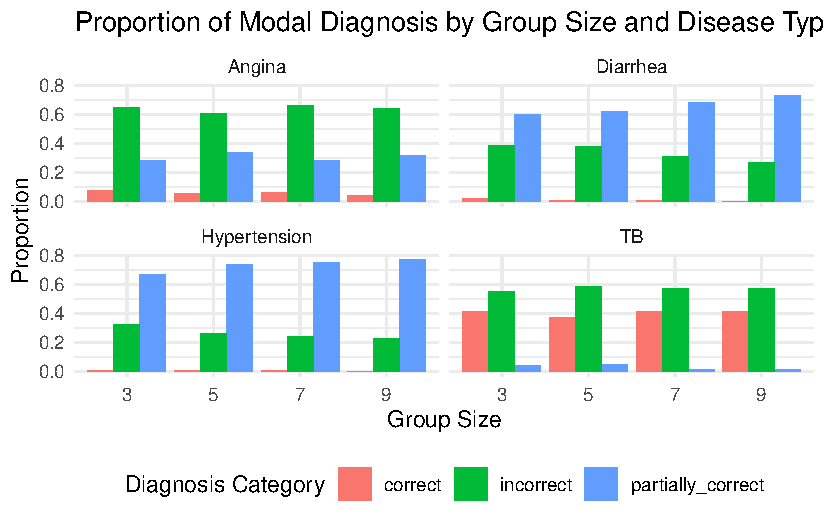
\includegraphics{simulation_files/figure-pdf/unnamed-chunk-3-1.pdf}

\subsubsection{2.1.3 Figure 2 - Simulation: 1PL IRT
model}\label{figure-2---simulation-1pl-irt-model}

\begin{Shaded}
\begin{Highlighting}[]
\CommentTok{\# Fix missing values in irtscore safely}
\NormalTok{visit\_data }\OtherTok{\textless{}{-}}\NormalTok{ visit\_data }\SpecialCharTok{\%\textgreater{}\%}
  \FunctionTok{mutate}\NormalTok{(}\AttributeTok{irtscore =} \FunctionTok{replace\_na}\NormalTok{(irtscore, }\FunctionTok{mean}\NormalTok{(irtscore, }\AttributeTok{na.rm =} \ConstantTok{TRUE}\NormalTok{)))}

\CommentTok{\# Function to compute weighted modal diagnosis with NA handling}
\NormalTok{compute\_weighted\_modal\_diagnosis }\OtherTok{\textless{}{-}} \ControlFlowTok{function}\NormalTok{(group) \{}
  \ControlFlowTok{if}\NormalTok{ (}\FunctionTok{nrow}\NormalTok{(group) }\SpecialCharTok{==} \DecValTok{0}\NormalTok{) }\FunctionTok{return}\NormalTok{(}\ConstantTok{NA}\NormalTok{)  }\CommentTok{\# Avoid missing values when group is empty}
  
\NormalTok{  weighted\_freq }\OtherTok{\textless{}{-}}\NormalTok{ group }\SpecialCharTok{\%\textgreater{}\%}
    \FunctionTok{group\_by}\NormalTok{(diagnosis) }\SpecialCharTok{\%\textgreater{}\%}
    \FunctionTok{summarise}\NormalTok{(}\AttributeTok{weighted\_sum =} \FunctionTok{sum}\NormalTok{(irtscore, }\AttributeTok{na.rm =} \ConstantTok{TRUE}\NormalTok{), }\AttributeTok{.groups =} \StringTok{"drop"}\NormalTok{) }\SpecialCharTok{\%\textgreater{}\%}
    \FunctionTok{arrange}\NormalTok{(}\FunctionTok{desc}\NormalTok{(weighted\_sum))}
  
  \CommentTok{\# Return most weighted diagnosis, or NA if none exists}
  \ControlFlowTok{if}\NormalTok{ (}\FunctionTok{nrow}\NormalTok{(weighted\_freq) }\SpecialCharTok{==} \DecValTok{0}\NormalTok{) }\FunctionTok{return}\NormalTok{(}\ConstantTok{NA}\NormalTok{)}
  \FunctionTok{return}\NormalTok{(weighted\_freq}\SpecialCharTok{$}\NormalTok{diagnosis[}\DecValTok{1}\NormalTok{])}
\NormalTok{\}}

\CommentTok{\# Simulation parameters}
\NormalTok{n\_simulations }\OtherTok{\textless{}{-}} \DecValTok{1000}
\NormalTok{group\_sizes }\OtherTok{\textless{}{-}} \FunctionTok{c}\NormalTok{(}\DecValTok{3}\NormalTok{, }\DecValTok{5}\NormalTok{, }\DecValTok{7}\NormalTok{, }\DecValTok{9}\NormalTok{)}

\CommentTok{\# Initialize a list to store results}
\NormalTok{results }\OtherTok{\textless{}{-}} \FunctionTok{list}\NormalTok{()}

\CommentTok{\# Run the simulation separately for each disease\_num}
\ControlFlowTok{for}\NormalTok{ (disease }\ControlFlowTok{in} \FunctionTok{unique}\NormalTok{(visit\_data}\SpecialCharTok{$}\NormalTok{disease\_num)) \{}
  \CommentTok{\# Filter data for the current disease\_num}
\NormalTok{  filtered\_data }\OtherTok{\textless{}{-}}\NormalTok{ visit\_data }\SpecialCharTok{\%\textgreater{}\%}
    \FunctionTok{filter}\NormalTok{(disease\_num }\SpecialCharTok{==}\NormalTok{ disease)}

  \ControlFlowTok{if}\NormalTok{ (}\FunctionTok{nrow}\NormalTok{(filtered\_data) }\SpecialCharTok{==} \DecValTok{0}\NormalTok{) }\ControlFlowTok{next}  \CommentTok{\# Skip if no data for this disease}
  
  \ControlFlowTok{for}\NormalTok{ (size }\ControlFlowTok{in}\NormalTok{ group\_sizes) \{}
    \ControlFlowTok{if}\NormalTok{ (}\FunctionTok{nrow}\NormalTok{(filtered\_data) }\SpecialCharTok{\textless{}}\NormalTok{ size) }\ControlFlowTok{next}  \CommentTok{\# Ensure enough cases for sampling}

\NormalTok{    proportions }\OtherTok{\textless{}{-}} \FunctionTok{data.frame}\NormalTok{(}
      \AttributeTok{simulation =} \FunctionTok{integer}\NormalTok{(),}
      \AttributeTok{correct =} \FunctionTok{numeric}\NormalTok{(),}
      \AttributeTok{partially\_correct =} \FunctionTok{numeric}\NormalTok{(),}
      \AttributeTok{incorrect =} \FunctionTok{numeric}\NormalTok{()}
\NormalTok{    )}
    
    \ControlFlowTok{for}\NormalTok{ (sim }\ControlFlowTok{in} \DecValTok{1}\SpecialCharTok{:}\NormalTok{n\_simulations) \{}
      \CommentTok{\# Randomly sample groups}
\NormalTok{      sampled\_groups }\OtherTok{\textless{}{-}}\NormalTok{ filtered\_data }\SpecialCharTok{\%\textgreater{}\%}
        \FunctionTok{sample\_n}\NormalTok{(}\AttributeTok{size =}\NormalTok{ size, }\AttributeTok{replace =} \ConstantTok{FALSE}\NormalTok{)}

      \CommentTok{\# Compute weighted modal diagnosis}
\NormalTok{      weighted\_modal\_diagnosis }\OtherTok{\textless{}{-}} \FunctionTok{compute\_weighted\_modal\_diagnosis}\NormalTok{(sampled\_groups)}

      \CommentTok{\# Handle missing weighted diagnosis (prevent NAs)}
      \ControlFlowTok{if}\NormalTok{ (}\FunctionTok{is.na}\NormalTok{(weighted\_modal\_diagnosis)) }\ControlFlowTok{next}  \CommentTok{\# Skip if modal diagnosis is missing}

      \CommentTok{\# Classify diagnosis}
\NormalTok{      diagnosis\_category }\OtherTok{\textless{}{-}} \FunctionTok{case\_when}\NormalTok{(}
\NormalTok{        weighted\_modal\_diagnosis }\SpecialCharTok{==} \DecValTok{2} \SpecialCharTok{\textasciitilde{}} \StringTok{"correct"}\NormalTok{,}
\NormalTok{        weighted\_modal\_diagnosis }\SpecialCharTok{==} \DecValTok{1} \SpecialCharTok{\textasciitilde{}} \StringTok{"partially\_correct"}\NormalTok{,}
\NormalTok{        weighted\_modal\_diagnosis }\SpecialCharTok{==} \DecValTok{0} \SpecialCharTok{\textasciitilde{}} \StringTok{"incorrect"}\NormalTok{,}
        \ConstantTok{TRUE} \SpecialCharTok{\textasciitilde{}} \ConstantTok{NA\_character\_}
\NormalTok{      )}

      \CommentTok{\# Ensure no NA in classification}
      \ControlFlowTok{if}\NormalTok{ (}\SpecialCharTok{!}\FunctionTok{is.na}\NormalTok{(diagnosis\_category)) \{}
\NormalTok{        proportions }\OtherTok{\textless{}{-}}\NormalTok{ proportions }\SpecialCharTok{\%\textgreater{}\%}
          \FunctionTok{add\_row}\NormalTok{(}
            \AttributeTok{simulation =}\NormalTok{ sim,}
            \AttributeTok{correct =} \FunctionTok{as.numeric}\NormalTok{(diagnosis\_category }\SpecialCharTok{==} \StringTok{"correct"}\NormalTok{),}
            \AttributeTok{partially\_correct =} \FunctionTok{as.numeric}\NormalTok{(diagnosis\_category }\SpecialCharTok{==} \StringTok{"partially\_correct"}\NormalTok{),}
            \AttributeTok{incorrect =} \FunctionTok{as.numeric}\NormalTok{(diagnosis\_category }\SpecialCharTok{==} \StringTok{"incorrect"}\NormalTok{)}
\NormalTok{          )}
\NormalTok{      \}}
\NormalTok{    \}}
    
    \CommentTok{\# Compute average proportions safely}
    \ControlFlowTok{if}\NormalTok{ (}\FunctionTok{nrow}\NormalTok{(proportions) }\SpecialCharTok{\textgreater{}} \DecValTok{0}\NormalTok{) \{}
\NormalTok{      avg\_proportions }\OtherTok{\textless{}{-}}\NormalTok{ proportions }\SpecialCharTok{\%\textgreater{}\%}
        \FunctionTok{summarise}\NormalTok{(}
          \AttributeTok{correct =} \FunctionTok{mean}\NormalTok{(correct, }\AttributeTok{na.rm =} \ConstantTok{TRUE}\NormalTok{),}
          \AttributeTok{partially\_correct =} \FunctionTok{mean}\NormalTok{(partially\_correct, }\AttributeTok{na.rm =} \ConstantTok{TRUE}\NormalTok{),}
          \AttributeTok{incorrect =} \FunctionTok{mean}\NormalTok{(incorrect, }\AttributeTok{na.rm =} \ConstantTok{TRUE}\NormalTok{)}
\NormalTok{        )}

      \CommentTok{\# Add metadata (group size and disease\_num)}
\NormalTok{      avg\_proportions}\SpecialCharTok{$}\NormalTok{group\_size }\OtherTok{\textless{}{-}}\NormalTok{ size}
\NormalTok{      avg\_proportions}\SpecialCharTok{$}\NormalTok{disease\_num }\OtherTok{\textless{}{-}}\NormalTok{ disease}

      \CommentTok{\# Store results}
\NormalTok{      results[[}\FunctionTok{paste}\NormalTok{(disease, size, }\AttributeTok{sep =} \StringTok{"\_"}\NormalTok{)]] }\OtherTok{\textless{}{-}}\NormalTok{ avg\_proportions}
\NormalTok{    \}}
\NormalTok{  \}}
\NormalTok{\}}

\CommentTok{\# Combine results into a single data frame}
\NormalTok{results\_df }\OtherTok{\textless{}{-}} \FunctionTok{bind\_rows}\NormalTok{(results)}

\CommentTok{\# Ensure no missing values in final data}
\NormalTok{results\_df }\OtherTok{\textless{}{-}}\NormalTok{ results\_df }\SpecialCharTok{\%\textgreater{}\%}
  \FunctionTok{drop\_na}\NormalTok{()}

\CommentTok{\# Reshape data for ggplot2}
\NormalTok{results\_long }\OtherTok{\textless{}{-}}\NormalTok{ results\_df }\SpecialCharTok{\%\textgreater{}\%}
  \FunctionTok{pivot\_longer}\NormalTok{(}\AttributeTok{cols =} \FunctionTok{c}\NormalTok{(correct, partially\_correct, incorrect),}
               \AttributeTok{names\_to =} \StringTok{"diagnosis\_category"}\NormalTok{,}
               \AttributeTok{values\_to =} \StringTok{"proportion"}\NormalTok{)}

\CommentTok{\# Plot the results}
\FunctionTok{ggplot}\NormalTok{(results\_long, }\FunctionTok{aes}\NormalTok{(}\AttributeTok{x =} \FunctionTok{factor}\NormalTok{(group\_size), }\AttributeTok{y =}\NormalTok{ proportion, }\AttributeTok{fill =}\NormalTok{ diagnosis\_category)) }\SpecialCharTok{+}
  \FunctionTok{geom\_bar}\NormalTok{(}\AttributeTok{stat =} \StringTok{"identity"}\NormalTok{, }\AttributeTok{position =} \StringTok{"dodge"}\NormalTok{) }\SpecialCharTok{+}
  \FunctionTok{facet\_wrap}\NormalTok{(}\SpecialCharTok{\textasciitilde{}}\NormalTok{disease\_num) }\SpecialCharTok{+}
  \FunctionTok{labs}\NormalTok{(}
    \AttributeTok{title =} \StringTok{"Proportion of Weighted Modal Diagnosis by Group Size and Disease Type"}\NormalTok{,}
    \AttributeTok{x =} \StringTok{"Group Size"}\NormalTok{,}
    \AttributeTok{y =} \StringTok{"Proportion"}\NormalTok{,}
    \AttributeTok{fill =} \StringTok{"Diagnosis Category"}
\NormalTok{  ) }\SpecialCharTok{+}
  \FunctionTok{theme\_minimal}\NormalTok{() }\SpecialCharTok{+}
  \FunctionTok{theme}\NormalTok{(}\AttributeTok{legend.position =} \StringTok{"bottom"}\NormalTok{)}
\end{Highlighting}
\end{Shaded}

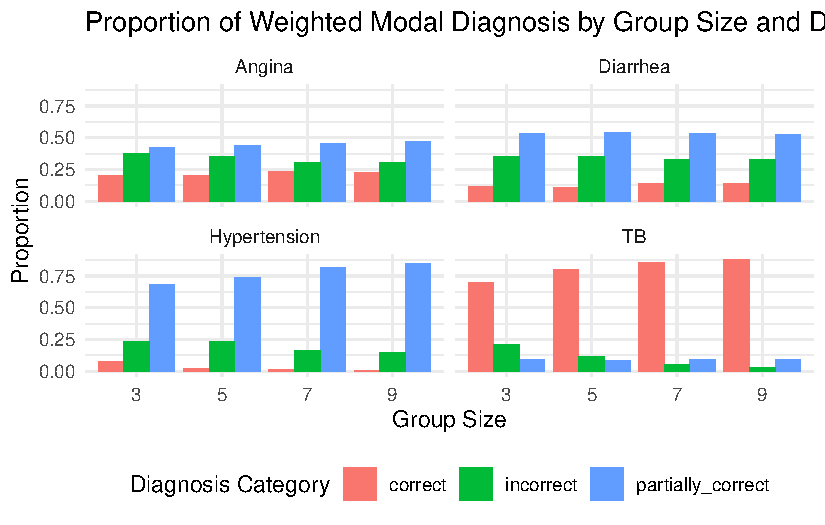
\includegraphics{simulation_files/figure-pdf/unnamed-chunk-4-1.pdf}

\subsubsection{2.1.4 Figure 3. New weighting method -
ML}\label{figure-3.-new-weighting-method---ml}

\begin{Shaded}
\begin{Highlighting}[]
\FunctionTok{library}\NormalTok{(caret)  }
\FunctionTok{library}\NormalTok{(randomForest)  }
\FunctionTok{library}\NormalTok{(xgboost)  }
\FunctionTok{library}\NormalTok{(nnet)  }
\FunctionTok{library}\NormalTok{(MLmetrics)}

\CommentTok{\# Prepare data for ML}
\NormalTok{ml\_data }\OtherTok{\textless{}{-}}\NormalTok{ visit\_data }\SpecialCharTok{\%\textgreater{}\%}
  \FunctionTok{select}\NormalTok{(diagnosis, irtscore) }\SpecialCharTok{\%\textgreater{}\%}
  \FunctionTok{filter}\NormalTok{(}\SpecialCharTok{!}\FunctionTok{is.na}\NormalTok{(diagnosis))  }\CommentTok{\# Remove rows with missing diagnosis}

\CommentTok{\# Convert diagnosis to a factor with valid names}
\NormalTok{ml\_data}\SpecialCharTok{$}\NormalTok{diagnosis }\OtherTok{\textless{}{-}} \FunctionTok{factor}\NormalTok{(ml\_data}\SpecialCharTok{$}\NormalTok{diagnosis, }\AttributeTok{labels =} \FunctionTok{c}\NormalTok{(}\StringTok{"Incorrect"}\NormalTok{, }\StringTok{"Partially\_Correct"}\NormalTok{, }\StringTok{"Correct"}\NormalTok{))}

\CommentTok{\# Split data into training and testing sets}
\FunctionTok{set.seed}\NormalTok{(}\DecValTok{2025}\NormalTok{)}
\NormalTok{train\_index }\OtherTok{\textless{}{-}} \FunctionTok{createDataPartition}\NormalTok{(ml\_data}\SpecialCharTok{$}\NormalTok{diagnosis, }\AttributeTok{p =} \FloatTok{0.8}\NormalTok{, }\AttributeTok{list =} \ConstantTok{FALSE}\NormalTok{)}
\NormalTok{train\_data }\OtherTok{\textless{}{-}}\NormalTok{ ml\_data[train\_index, ]}
\NormalTok{test\_data }\OtherTok{\textless{}{-}}\NormalTok{ ml\_data[}\SpecialCharTok{{-}}\NormalTok{train\_index, ]}

\CommentTok{\# Define model training control}
\NormalTok{control }\OtherTok{\textless{}{-}} \FunctionTok{trainControl}\NormalTok{(}\AttributeTok{method =} \StringTok{"cv"}\NormalTok{, }\AttributeTok{number =} \DecValTok{5}\NormalTok{, }\AttributeTok{classProbs =} \ConstantTok{TRUE}\NormalTok{, }\AttributeTok{summaryFunction =}\NormalTok{ multiClassSummary)}

\CommentTok{\# Train multiple ML models (classification)}
\FunctionTok{set.seed}\NormalTok{(}\DecValTok{2025}\NormalTok{)}
\NormalTok{models }\OtherTok{\textless{}{-}} \FunctionTok{list}\NormalTok{(}
  \AttributeTok{logistic =} \FunctionTok{train}\NormalTok{(diagnosis }\SpecialCharTok{\textasciitilde{}}\NormalTok{ irtscore, }\AttributeTok{data =}\NormalTok{ train\_data, }
                   \AttributeTok{method =} \ControlFlowTok{if}\NormalTok{ (}\FunctionTok{length}\NormalTok{(}\FunctionTok{levels}\NormalTok{(train\_data}\SpecialCharTok{$}\NormalTok{diagnosis)) }\SpecialCharTok{\textgreater{}} \DecValTok{2}\NormalTok{) }\StringTok{"multinom"} \ControlFlowTok{else} \StringTok{"glm"}\NormalTok{, }
                   \AttributeTok{family =} \ControlFlowTok{if}\NormalTok{ (}\FunctionTok{length}\NormalTok{(}\FunctionTok{levels}\NormalTok{(train\_data}\SpecialCharTok{$}\NormalTok{diagnosis)) }\SpecialCharTok{\textgreater{}} \DecValTok{2}\NormalTok{) }\ConstantTok{NULL} \ControlFlowTok{else} \StringTok{"binomial"}\NormalTok{, }
                   \AttributeTok{trControl =}\NormalTok{ control),}
  
  \AttributeTok{random\_forest =} \FunctionTok{train}\NormalTok{(diagnosis }\SpecialCharTok{\textasciitilde{}}\NormalTok{ irtscore, }\AttributeTok{data =}\NormalTok{ train\_data, }
                        \AttributeTok{method =} \StringTok{"rf"}\NormalTok{, }
                        \AttributeTok{trControl =}\NormalTok{ control),}
  
  \AttributeTok{xgboost =} \FunctionTok{train}\NormalTok{(diagnosis }\SpecialCharTok{\textasciitilde{}}\NormalTok{ irtscore, }\AttributeTok{data =}\NormalTok{ train\_data, }
                  \AttributeTok{method =} \StringTok{"xgbTree"}\NormalTok{, }
                  \AttributeTok{trControl =}\NormalTok{ control)}
\NormalTok{)}
\end{Highlighting}
\end{Shaded}

\begin{verbatim}
# weights:  9 (4 variable)
initial  value 1790.738031 
iter  10 value 1639.418641
iter  10 value 1639.418641
final  value 1639.418641 
converged
# weights:  9 (4 variable)
initial  value 1790.738031 
iter  10 value 1639.530715
iter  10 value 1639.530715
final  value 1639.530715 
converged
# weights:  9 (4 variable)
initial  value 1790.738031 
iter  10 value 1639.418753
iter  10 value 1639.418753
final  value 1639.418753 
converged
# weights:  9 (4 variable)
initial  value 1791.836643 
iter  10 value 1646.173715
iter  10 value 1646.173715
final  value 1646.173715 
converged
# weights:  9 (4 variable)
initial  value 1791.836643 
final  value 1646.280190 
converged
# weights:  9 (4 variable)
initial  value 1791.836643 
iter  10 value 1646.173822
iter  10 value 1646.173822
final  value 1646.173822 
converged
# weights:  9 (4 variable)
initial  value 1791.836643 
final  value 1644.710855 
converged
# weights:  9 (4 variable)
initial  value 1791.836643 
final  value 1644.818041 
converged
# weights:  9 (4 variable)
initial  value 1791.836643 
final  value 1644.710962 
converged
# weights:  9 (4 variable)
initial  value 1791.836643 
iter  10 value 1641.388957
iter  10 value 1641.388956
final  value 1641.388956 
converged
# weights:  9 (4 variable)
initial  value 1791.836643 
iter  10 value 1641.510980
iter  10 value 1641.510979
final  value 1641.510979 
converged
# weights:  9 (4 variable)
initial  value 1791.836643 
iter  10 value 1641.389079
iter  10 value 1641.389079
final  value 1641.389079 
converged
# weights:  9 (4 variable)
initial  value 1794.033867 
iter  10 value 1643.151091
iter  10 value 1643.151081
final  value 1643.151081 
converged
# weights:  9 (4 variable)
initial  value 1794.033867 
iter  10 value 1643.271090
iter  10 value 1643.271078
final  value 1643.271078 
converged
# weights:  9 (4 variable)
initial  value 1794.033867 
iter  10 value 1643.151211
iter  10 value 1643.151201
final  value 1643.151201 
converged
\end{verbatim}

\begin{verbatim}
# weights:  9 (4 variable)
initial  value 2240.070457 
final  value 2054.197843 
converged
\end{verbatim}

\begin{verbatim}
[00:52:32] WARNING: src/c_api/c_api.cc:935: `ntree_limit` is deprecated, use `iteration_range` instead.
[00:52:32] WARNING: src/c_api/c_api.cc:935: `ntree_limit` is deprecated, use `iteration_range` instead.
[00:52:32] WARNING: src/c_api/c_api.cc:935: `ntree_limit` is deprecated, use `iteration_range` instead.
[00:52:32] WARNING: src/c_api/c_api.cc:935: `ntree_limit` is deprecated, use `iteration_range` instead.
[00:52:33] WARNING: src/c_api/c_api.cc:935: `ntree_limit` is deprecated, use `iteration_range` instead.
[00:52:33] WARNING: src/c_api/c_api.cc:935: `ntree_limit` is deprecated, use `iteration_range` instead.
[00:52:33] WARNING: src/c_api/c_api.cc:935: `ntree_limit` is deprecated, use `iteration_range` instead.
[00:52:33] WARNING: src/c_api/c_api.cc:935: `ntree_limit` is deprecated, use `iteration_range` instead.
[00:52:33] WARNING: src/c_api/c_api.cc:935: `ntree_limit` is deprecated, use `iteration_range` instead.
[00:52:33] WARNING: src/c_api/c_api.cc:935: `ntree_limit` is deprecated, use `iteration_range` instead.
[00:52:33] WARNING: src/c_api/c_api.cc:935: `ntree_limit` is deprecated, use `iteration_range` instead.
[00:52:33] WARNING: src/c_api/c_api.cc:935: `ntree_limit` is deprecated, use `iteration_range` instead.
[00:52:33] WARNING: src/c_api/c_api.cc:935: `ntree_limit` is deprecated, use `iteration_range` instead.
[00:52:33] WARNING: src/c_api/c_api.cc:935: `ntree_limit` is deprecated, use `iteration_range` instead.
[00:52:33] WARNING: src/c_api/c_api.cc:935: `ntree_limit` is deprecated, use `iteration_range` instead.
[00:52:33] WARNING: src/c_api/c_api.cc:935: `ntree_limit` is deprecated, use `iteration_range` instead.
[00:52:33] WARNING: src/c_api/c_api.cc:935: `ntree_limit` is deprecated, use `iteration_range` instead.
[00:52:33] WARNING: src/c_api/c_api.cc:935: `ntree_limit` is deprecated, use `iteration_range` instead.
[00:52:33] WARNING: src/c_api/c_api.cc:935: `ntree_limit` is deprecated, use `iteration_range` instead.
[00:52:33] WARNING: src/c_api/c_api.cc:935: `ntree_limit` is deprecated, use `iteration_range` instead.
[00:52:33] WARNING: src/c_api/c_api.cc:935: `ntree_limit` is deprecated, use `iteration_range` instead.
[00:52:33] WARNING: src/c_api/c_api.cc:935: `ntree_limit` is deprecated, use `iteration_range` instead.
[00:52:33] WARNING: src/c_api/c_api.cc:935: `ntree_limit` is deprecated, use `iteration_range` instead.
[00:52:33] WARNING: src/c_api/c_api.cc:935: `ntree_limit` is deprecated, use `iteration_range` instead.
[00:52:33] WARNING: src/c_api/c_api.cc:935: `ntree_limit` is deprecated, use `iteration_range` instead.
[00:52:33] WARNING: src/c_api/c_api.cc:935: `ntree_limit` is deprecated, use `iteration_range` instead.
[00:52:33] WARNING: src/c_api/c_api.cc:935: `ntree_limit` is deprecated, use `iteration_range` instead.
[00:52:33] WARNING: src/c_api/c_api.cc:935: `ntree_limit` is deprecated, use `iteration_range` instead.
[00:52:33] WARNING: src/c_api/c_api.cc:935: `ntree_limit` is deprecated, use `iteration_range` instead.
[00:52:33] WARNING: src/c_api/c_api.cc:935: `ntree_limit` is deprecated, use `iteration_range` instead.
[00:52:33] WARNING: src/c_api/c_api.cc:935: `ntree_limit` is deprecated, use `iteration_range` instead.
[00:52:33] WARNING: src/c_api/c_api.cc:935: `ntree_limit` is deprecated, use `iteration_range` instead.
[00:52:33] WARNING: src/c_api/c_api.cc:935: `ntree_limit` is deprecated, use `iteration_range` instead.
[00:52:33] WARNING: src/c_api/c_api.cc:935: `ntree_limit` is deprecated, use `iteration_range` instead.
[00:52:33] WARNING: src/c_api/c_api.cc:935: `ntree_limit` is deprecated, use `iteration_range` instead.
[00:52:33] WARNING: src/c_api/c_api.cc:935: `ntree_limit` is deprecated, use `iteration_range` instead.
[00:52:33] WARNING: src/c_api/c_api.cc:935: `ntree_limit` is deprecated, use `iteration_range` instead.
[00:52:33] WARNING: src/c_api/c_api.cc:935: `ntree_limit` is deprecated, use `iteration_range` instead.
[00:52:33] WARNING: src/c_api/c_api.cc:935: `ntree_limit` is deprecated, use `iteration_range` instead.
[00:52:33] WARNING: src/c_api/c_api.cc:935: `ntree_limit` is deprecated, use `iteration_range` instead.
[00:52:33] WARNING: src/c_api/c_api.cc:935: `ntree_limit` is deprecated, use `iteration_range` instead.
[00:52:33] WARNING: src/c_api/c_api.cc:935: `ntree_limit` is deprecated, use `iteration_range` instead.
[00:52:33] WARNING: src/c_api/c_api.cc:935: `ntree_limit` is deprecated, use `iteration_range` instead.
[00:52:33] WARNING: src/c_api/c_api.cc:935: `ntree_limit` is deprecated, use `iteration_range` instead.
[00:52:33] WARNING: src/c_api/c_api.cc:935: `ntree_limit` is deprecated, use `iteration_range` instead.
[00:52:33] WARNING: src/c_api/c_api.cc:935: `ntree_limit` is deprecated, use `iteration_range` instead.
[00:52:33] WARNING: src/c_api/c_api.cc:935: `ntree_limit` is deprecated, use `iteration_range` instead.
[00:52:33] WARNING: src/c_api/c_api.cc:935: `ntree_limit` is deprecated, use `iteration_range` instead.
[00:52:33] WARNING: src/c_api/c_api.cc:935: `ntree_limit` is deprecated, use `iteration_range` instead.
[00:52:33] WARNING: src/c_api/c_api.cc:935: `ntree_limit` is deprecated, use `iteration_range` instead.
[00:52:33] WARNING: src/c_api/c_api.cc:935: `ntree_limit` is deprecated, use `iteration_range` instead.
[00:52:33] WARNING: src/c_api/c_api.cc:935: `ntree_limit` is deprecated, use `iteration_range` instead.
[00:52:34] WARNING: src/c_api/c_api.cc:935: `ntree_limit` is deprecated, use `iteration_range` instead.
[00:52:34] WARNING: src/c_api/c_api.cc:935: `ntree_limit` is deprecated, use `iteration_range` instead.
[00:52:34] WARNING: src/c_api/c_api.cc:935: `ntree_limit` is deprecated, use `iteration_range` instead.
[00:52:34] WARNING: src/c_api/c_api.cc:935: `ntree_limit` is deprecated, use `iteration_range` instead.
[00:52:34] WARNING: src/c_api/c_api.cc:935: `ntree_limit` is deprecated, use `iteration_range` instead.
[00:52:34] WARNING: src/c_api/c_api.cc:935: `ntree_limit` is deprecated, use `iteration_range` instead.
[00:52:34] WARNING: src/c_api/c_api.cc:935: `ntree_limit` is deprecated, use `iteration_range` instead.
[00:52:34] WARNING: src/c_api/c_api.cc:935: `ntree_limit` is deprecated, use `iteration_range` instead.
[00:52:34] WARNING: src/c_api/c_api.cc:935: `ntree_limit` is deprecated, use `iteration_range` instead.
[00:52:34] WARNING: src/c_api/c_api.cc:935: `ntree_limit` is deprecated, use `iteration_range` instead.
[00:52:34] WARNING: src/c_api/c_api.cc:935: `ntree_limit` is deprecated, use `iteration_range` instead.
[00:52:34] WARNING: src/c_api/c_api.cc:935: `ntree_limit` is deprecated, use `iteration_range` instead.
[00:52:34] WARNING: src/c_api/c_api.cc:935: `ntree_limit` is deprecated, use `iteration_range` instead.
[00:52:34] WARNING: src/c_api/c_api.cc:935: `ntree_limit` is deprecated, use `iteration_range` instead.
[00:52:34] WARNING: src/c_api/c_api.cc:935: `ntree_limit` is deprecated, use `iteration_range` instead.
[00:52:34] WARNING: src/c_api/c_api.cc:935: `ntree_limit` is deprecated, use `iteration_range` instead.
[00:52:34] WARNING: src/c_api/c_api.cc:935: `ntree_limit` is deprecated, use `iteration_range` instead.
[00:52:34] WARNING: src/c_api/c_api.cc:935: `ntree_limit` is deprecated, use `iteration_range` instead.
[00:52:34] WARNING: src/c_api/c_api.cc:935: `ntree_limit` is deprecated, use `iteration_range` instead.
[00:52:34] WARNING: src/c_api/c_api.cc:935: `ntree_limit` is deprecated, use `iteration_range` instead.
[00:52:34] WARNING: src/c_api/c_api.cc:935: `ntree_limit` is deprecated, use `iteration_range` instead.
[00:52:34] WARNING: src/c_api/c_api.cc:935: `ntree_limit` is deprecated, use `iteration_range` instead.
[00:52:34] WARNING: src/c_api/c_api.cc:935: `ntree_limit` is deprecated, use `iteration_range` instead.
[00:52:34] WARNING: src/c_api/c_api.cc:935: `ntree_limit` is deprecated, use `iteration_range` instead.
[00:52:34] WARNING: src/c_api/c_api.cc:935: `ntree_limit` is deprecated, use `iteration_range` instead.
[00:52:34] WARNING: src/c_api/c_api.cc:935: `ntree_limit` is deprecated, use `iteration_range` instead.
[00:52:34] WARNING: src/c_api/c_api.cc:935: `ntree_limit` is deprecated, use `iteration_range` instead.
[00:52:34] WARNING: src/c_api/c_api.cc:935: `ntree_limit` is deprecated, use `iteration_range` instead.
[00:52:34] WARNING: src/c_api/c_api.cc:935: `ntree_limit` is deprecated, use `iteration_range` instead.
[00:52:34] WARNING: src/c_api/c_api.cc:935: `ntree_limit` is deprecated, use `iteration_range` instead.
[00:52:34] WARNING: src/c_api/c_api.cc:935: `ntree_limit` is deprecated, use `iteration_range` instead.
[00:52:34] WARNING: src/c_api/c_api.cc:935: `ntree_limit` is deprecated, use `iteration_range` instead.
[00:52:34] WARNING: src/c_api/c_api.cc:935: `ntree_limit` is deprecated, use `iteration_range` instead.
[00:52:34] WARNING: src/c_api/c_api.cc:935: `ntree_limit` is deprecated, use `iteration_range` instead.
[00:52:34] WARNING: src/c_api/c_api.cc:935: `ntree_limit` is deprecated, use `iteration_range` instead.
[00:52:34] WARNING: src/c_api/c_api.cc:935: `ntree_limit` is deprecated, use `iteration_range` instead.
[00:52:34] WARNING: src/c_api/c_api.cc:935: `ntree_limit` is deprecated, use `iteration_range` instead.
[00:52:34] WARNING: src/c_api/c_api.cc:935: `ntree_limit` is deprecated, use `iteration_range` instead.
[00:52:34] WARNING: src/c_api/c_api.cc:935: `ntree_limit` is deprecated, use `iteration_range` instead.
[00:52:34] WARNING: src/c_api/c_api.cc:935: `ntree_limit` is deprecated, use `iteration_range` instead.
[00:52:34] WARNING: src/c_api/c_api.cc:935: `ntree_limit` is deprecated, use `iteration_range` instead.
[00:52:34] WARNING: src/c_api/c_api.cc:935: `ntree_limit` is deprecated, use `iteration_range` instead.
[00:52:34] WARNING: src/c_api/c_api.cc:935: `ntree_limit` is deprecated, use `iteration_range` instead.
[00:52:34] WARNING: src/c_api/c_api.cc:935: `ntree_limit` is deprecated, use `iteration_range` instead.
[00:52:35] WARNING: src/c_api/c_api.cc:935: `ntree_limit` is deprecated, use `iteration_range` instead.
[00:52:35] WARNING: src/c_api/c_api.cc:935: `ntree_limit` is deprecated, use `iteration_range` instead.
[00:52:35] WARNING: src/c_api/c_api.cc:935: `ntree_limit` is deprecated, use `iteration_range` instead.
[00:52:35] WARNING: src/c_api/c_api.cc:935: `ntree_limit` is deprecated, use `iteration_range` instead.
[00:52:35] WARNING: src/c_api/c_api.cc:935: `ntree_limit` is deprecated, use `iteration_range` instead.
[00:52:35] WARNING: src/c_api/c_api.cc:935: `ntree_limit` is deprecated, use `iteration_range` instead.
[00:52:35] WARNING: src/c_api/c_api.cc:935: `ntree_limit` is deprecated, use `iteration_range` instead.
[00:52:35] WARNING: src/c_api/c_api.cc:935: `ntree_limit` is deprecated, use `iteration_range` instead.
[00:52:35] WARNING: src/c_api/c_api.cc:935: `ntree_limit` is deprecated, use `iteration_range` instead.
[00:52:35] WARNING: src/c_api/c_api.cc:935: `ntree_limit` is deprecated, use `iteration_range` instead.
[00:52:35] WARNING: src/c_api/c_api.cc:935: `ntree_limit` is deprecated, use `iteration_range` instead.
[00:52:35] WARNING: src/c_api/c_api.cc:935: `ntree_limit` is deprecated, use `iteration_range` instead.
[00:52:35] WARNING: src/c_api/c_api.cc:935: `ntree_limit` is deprecated, use `iteration_range` instead.
[00:52:35] WARNING: src/c_api/c_api.cc:935: `ntree_limit` is deprecated, use `iteration_range` instead.
[00:52:35] WARNING: src/c_api/c_api.cc:935: `ntree_limit` is deprecated, use `iteration_range` instead.
[00:52:35] WARNING: src/c_api/c_api.cc:935: `ntree_limit` is deprecated, use `iteration_range` instead.
[00:52:35] WARNING: src/c_api/c_api.cc:935: `ntree_limit` is deprecated, use `iteration_range` instead.
[00:52:35] WARNING: src/c_api/c_api.cc:935: `ntree_limit` is deprecated, use `iteration_range` instead.
[00:52:35] WARNING: src/c_api/c_api.cc:935: `ntree_limit` is deprecated, use `iteration_range` instead.
[00:52:35] WARNING: src/c_api/c_api.cc:935: `ntree_limit` is deprecated, use `iteration_range` instead.
[00:52:35] WARNING: src/c_api/c_api.cc:935: `ntree_limit` is deprecated, use `iteration_range` instead.
[00:52:35] WARNING: src/c_api/c_api.cc:935: `ntree_limit` is deprecated, use `iteration_range` instead.
[00:52:35] WARNING: src/c_api/c_api.cc:935: `ntree_limit` is deprecated, use `iteration_range` instead.
[00:52:35] WARNING: src/c_api/c_api.cc:935: `ntree_limit` is deprecated, use `iteration_range` instead.
[00:52:35] WARNING: src/c_api/c_api.cc:935: `ntree_limit` is deprecated, use `iteration_range` instead.
[00:52:35] WARNING: src/c_api/c_api.cc:935: `ntree_limit` is deprecated, use `iteration_range` instead.
[00:52:35] WARNING: src/c_api/c_api.cc:935: `ntree_limit` is deprecated, use `iteration_range` instead.
[00:52:35] WARNING: src/c_api/c_api.cc:935: `ntree_limit` is deprecated, use `iteration_range` instead.
[00:52:35] WARNING: src/c_api/c_api.cc:935: `ntree_limit` is deprecated, use `iteration_range` instead.
[00:52:35] WARNING: src/c_api/c_api.cc:935: `ntree_limit` is deprecated, use `iteration_range` instead.
[00:52:35] WARNING: src/c_api/c_api.cc:935: `ntree_limit` is deprecated, use `iteration_range` instead.
[00:52:35] WARNING: src/c_api/c_api.cc:935: `ntree_limit` is deprecated, use `iteration_range` instead.
[00:52:35] WARNING: src/c_api/c_api.cc:935: `ntree_limit` is deprecated, use `iteration_range` instead.
[00:52:35] WARNING: src/c_api/c_api.cc:935: `ntree_limit` is deprecated, use `iteration_range` instead.
[00:52:35] WARNING: src/c_api/c_api.cc:935: `ntree_limit` is deprecated, use `iteration_range` instead.
[00:52:35] WARNING: src/c_api/c_api.cc:935: `ntree_limit` is deprecated, use `iteration_range` instead.
[00:52:36] WARNING: src/c_api/c_api.cc:935: `ntree_limit` is deprecated, use `iteration_range` instead.
[00:52:36] WARNING: src/c_api/c_api.cc:935: `ntree_limit` is deprecated, use `iteration_range` instead.
[00:52:36] WARNING: src/c_api/c_api.cc:935: `ntree_limit` is deprecated, use `iteration_range` instead.
[00:52:36] WARNING: src/c_api/c_api.cc:935: `ntree_limit` is deprecated, use `iteration_range` instead.
[00:52:36] WARNING: src/c_api/c_api.cc:935: `ntree_limit` is deprecated, use `iteration_range` instead.
[00:52:36] WARNING: src/c_api/c_api.cc:935: `ntree_limit` is deprecated, use `iteration_range` instead.
[00:52:36] WARNING: src/c_api/c_api.cc:935: `ntree_limit` is deprecated, use `iteration_range` instead.
[00:52:36] WARNING: src/c_api/c_api.cc:935: `ntree_limit` is deprecated, use `iteration_range` instead.
[00:52:36] WARNING: src/c_api/c_api.cc:935: `ntree_limit` is deprecated, use `iteration_range` instead.
[00:52:36] WARNING: src/c_api/c_api.cc:935: `ntree_limit` is deprecated, use `iteration_range` instead.
[00:52:36] WARNING: src/c_api/c_api.cc:935: `ntree_limit` is deprecated, use `iteration_range` instead.
[00:52:36] WARNING: src/c_api/c_api.cc:935: `ntree_limit` is deprecated, use `iteration_range` instead.
[00:52:36] WARNING: src/c_api/c_api.cc:935: `ntree_limit` is deprecated, use `iteration_range` instead.
[00:52:36] WARNING: src/c_api/c_api.cc:935: `ntree_limit` is deprecated, use `iteration_range` instead.
[00:52:36] WARNING: src/c_api/c_api.cc:935: `ntree_limit` is deprecated, use `iteration_range` instead.
[00:52:36] WARNING: src/c_api/c_api.cc:935: `ntree_limit` is deprecated, use `iteration_range` instead.
[00:52:36] WARNING: src/c_api/c_api.cc:935: `ntree_limit` is deprecated, use `iteration_range` instead.
[00:52:36] WARNING: src/c_api/c_api.cc:935: `ntree_limit` is deprecated, use `iteration_range` instead.
[00:52:36] WARNING: src/c_api/c_api.cc:935: `ntree_limit` is deprecated, use `iteration_range` instead.
[00:52:36] WARNING: src/c_api/c_api.cc:935: `ntree_limit` is deprecated, use `iteration_range` instead.
[00:52:36] WARNING: src/c_api/c_api.cc:935: `ntree_limit` is deprecated, use `iteration_range` instead.
[00:52:36] WARNING: src/c_api/c_api.cc:935: `ntree_limit` is deprecated, use `iteration_range` instead.
[00:52:36] WARNING: src/c_api/c_api.cc:935: `ntree_limit` is deprecated, use `iteration_range` instead.
[00:52:36] WARNING: src/c_api/c_api.cc:935: `ntree_limit` is deprecated, use `iteration_range` instead.
[00:52:36] WARNING: src/c_api/c_api.cc:935: `ntree_limit` is deprecated, use `iteration_range` instead.
[00:52:36] WARNING: src/c_api/c_api.cc:935: `ntree_limit` is deprecated, use `iteration_range` instead.
[00:52:36] WARNING: src/c_api/c_api.cc:935: `ntree_limit` is deprecated, use `iteration_range` instead.
[00:52:36] WARNING: src/c_api/c_api.cc:935: `ntree_limit` is deprecated, use `iteration_range` instead.
[00:52:36] WARNING: src/c_api/c_api.cc:935: `ntree_limit` is deprecated, use `iteration_range` instead.
[00:52:36] WARNING: src/c_api/c_api.cc:935: `ntree_limit` is deprecated, use `iteration_range` instead.
[00:52:36] WARNING: src/c_api/c_api.cc:935: `ntree_limit` is deprecated, use `iteration_range` instead.
[00:52:36] WARNING: src/c_api/c_api.cc:935: `ntree_limit` is deprecated, use `iteration_range` instead.
[00:52:36] WARNING: src/c_api/c_api.cc:935: `ntree_limit` is deprecated, use `iteration_range` instead.
[00:52:36] WARNING: src/c_api/c_api.cc:935: `ntree_limit` is deprecated, use `iteration_range` instead.
[00:52:36] WARNING: src/c_api/c_api.cc:935: `ntree_limit` is deprecated, use `iteration_range` instead.
[00:52:36] WARNING: src/c_api/c_api.cc:935: `ntree_limit` is deprecated, use `iteration_range` instead.
[00:52:36] WARNING: src/c_api/c_api.cc:935: `ntree_limit` is deprecated, use `iteration_range` instead.
[00:52:36] WARNING: src/c_api/c_api.cc:935: `ntree_limit` is deprecated, use `iteration_range` instead.
[00:52:36] WARNING: src/c_api/c_api.cc:935: `ntree_limit` is deprecated, use `iteration_range` instead.
[00:52:36] WARNING: src/c_api/c_api.cc:935: `ntree_limit` is deprecated, use `iteration_range` instead.
[00:52:36] WARNING: src/c_api/c_api.cc:935: `ntree_limit` is deprecated, use `iteration_range` instead.
[00:52:36] WARNING: src/c_api/c_api.cc:935: `ntree_limit` is deprecated, use `iteration_range` instead.
[00:52:36] WARNING: src/c_api/c_api.cc:935: `ntree_limit` is deprecated, use `iteration_range` instead.
[00:52:36] WARNING: src/c_api/c_api.cc:935: `ntree_limit` is deprecated, use `iteration_range` instead.
[00:52:36] WARNING: src/c_api/c_api.cc:935: `ntree_limit` is deprecated, use `iteration_range` instead.
[00:52:36] WARNING: src/c_api/c_api.cc:935: `ntree_limit` is deprecated, use `iteration_range` instead.
[00:52:36] WARNING: src/c_api/c_api.cc:935: `ntree_limit` is deprecated, use `iteration_range` instead.
[00:52:36] WARNING: src/c_api/c_api.cc:935: `ntree_limit` is deprecated, use `iteration_range` instead.
[00:52:37] WARNING: src/c_api/c_api.cc:935: `ntree_limit` is deprecated, use `iteration_range` instead.
[00:52:37] WARNING: src/c_api/c_api.cc:935: `ntree_limit` is deprecated, use `iteration_range` instead.
[00:52:37] WARNING: src/c_api/c_api.cc:935: `ntree_limit` is deprecated, use `iteration_range` instead.
[00:52:37] WARNING: src/c_api/c_api.cc:935: `ntree_limit` is deprecated, use `iteration_range` instead.
[00:52:37] WARNING: src/c_api/c_api.cc:935: `ntree_limit` is deprecated, use `iteration_range` instead.
[00:52:37] WARNING: src/c_api/c_api.cc:935: `ntree_limit` is deprecated, use `iteration_range` instead.
[00:52:37] WARNING: src/c_api/c_api.cc:935: `ntree_limit` is deprecated, use `iteration_range` instead.
[00:52:37] WARNING: src/c_api/c_api.cc:935: `ntree_limit` is deprecated, use `iteration_range` instead.
[00:52:37] WARNING: src/c_api/c_api.cc:935: `ntree_limit` is deprecated, use `iteration_range` instead.
[00:52:37] WARNING: src/c_api/c_api.cc:935: `ntree_limit` is deprecated, use `iteration_range` instead.
[00:52:37] WARNING: src/c_api/c_api.cc:935: `ntree_limit` is deprecated, use `iteration_range` instead.
[00:52:37] WARNING: src/c_api/c_api.cc:935: `ntree_limit` is deprecated, use `iteration_range` instead.
[00:52:37] WARNING: src/c_api/c_api.cc:935: `ntree_limit` is deprecated, use `iteration_range` instead.
[00:52:37] WARNING: src/c_api/c_api.cc:935: `ntree_limit` is deprecated, use `iteration_range` instead.
[00:52:37] WARNING: src/c_api/c_api.cc:935: `ntree_limit` is deprecated, use `iteration_range` instead.
[00:52:37] WARNING: src/c_api/c_api.cc:935: `ntree_limit` is deprecated, use `iteration_range` instead.
[00:52:37] WARNING: src/c_api/c_api.cc:935: `ntree_limit` is deprecated, use `iteration_range` instead.
[00:52:37] WARNING: src/c_api/c_api.cc:935: `ntree_limit` is deprecated, use `iteration_range` instead.
[00:52:37] WARNING: src/c_api/c_api.cc:935: `ntree_limit` is deprecated, use `iteration_range` instead.
[00:52:37] WARNING: src/c_api/c_api.cc:935: `ntree_limit` is deprecated, use `iteration_range` instead.
[00:52:37] WARNING: src/c_api/c_api.cc:935: `ntree_limit` is deprecated, use `iteration_range` instead.
[00:52:37] WARNING: src/c_api/c_api.cc:935: `ntree_limit` is deprecated, use `iteration_range` instead.
[00:52:37] WARNING: src/c_api/c_api.cc:935: `ntree_limit` is deprecated, use `iteration_range` instead.
[00:52:37] WARNING: src/c_api/c_api.cc:935: `ntree_limit` is deprecated, use `iteration_range` instead.
[00:52:37] WARNING: src/c_api/c_api.cc:935: `ntree_limit` is deprecated, use `iteration_range` instead.
[00:52:37] WARNING: src/c_api/c_api.cc:935: `ntree_limit` is deprecated, use `iteration_range` instead.
[00:52:37] WARNING: src/c_api/c_api.cc:935: `ntree_limit` is deprecated, use `iteration_range` instead.
[00:52:37] WARNING: src/c_api/c_api.cc:935: `ntree_limit` is deprecated, use `iteration_range` instead.
[00:52:37] WARNING: src/c_api/c_api.cc:935: `ntree_limit` is deprecated, use `iteration_range` instead.
[00:52:37] WARNING: src/c_api/c_api.cc:935: `ntree_limit` is deprecated, use `iteration_range` instead.
[00:52:37] WARNING: src/c_api/c_api.cc:935: `ntree_limit` is deprecated, use `iteration_range` instead.
[00:52:37] WARNING: src/c_api/c_api.cc:935: `ntree_limit` is deprecated, use `iteration_range` instead.
[00:52:37] WARNING: src/c_api/c_api.cc:935: `ntree_limit` is deprecated, use `iteration_range` instead.
[00:52:37] WARNING: src/c_api/c_api.cc:935: `ntree_limit` is deprecated, use `iteration_range` instead.
[00:52:37] WARNING: src/c_api/c_api.cc:935: `ntree_limit` is deprecated, use `iteration_range` instead.
[00:52:37] WARNING: src/c_api/c_api.cc:935: `ntree_limit` is deprecated, use `iteration_range` instead.
[00:52:37] WARNING: src/c_api/c_api.cc:935: `ntree_limit` is deprecated, use `iteration_range` instead.
[00:52:37] WARNING: src/c_api/c_api.cc:935: `ntree_limit` is deprecated, use `iteration_range` instead.
[00:52:37] WARNING: src/c_api/c_api.cc:935: `ntree_limit` is deprecated, use `iteration_range` instead.
[00:52:37] WARNING: src/c_api/c_api.cc:935: `ntree_limit` is deprecated, use `iteration_range` instead.
[00:52:38] WARNING: src/c_api/c_api.cc:935: `ntree_limit` is deprecated, use `iteration_range` instead.
[00:52:38] WARNING: src/c_api/c_api.cc:935: `ntree_limit` is deprecated, use `iteration_range` instead.
[00:52:38] WARNING: src/c_api/c_api.cc:935: `ntree_limit` is deprecated, use `iteration_range` instead.
[00:52:38] WARNING: src/c_api/c_api.cc:935: `ntree_limit` is deprecated, use `iteration_range` instead.
[00:52:38] WARNING: src/c_api/c_api.cc:935: `ntree_limit` is deprecated, use `iteration_range` instead.
[00:52:38] WARNING: src/c_api/c_api.cc:935: `ntree_limit` is deprecated, use `iteration_range` instead.
[00:52:38] WARNING: src/c_api/c_api.cc:935: `ntree_limit` is deprecated, use `iteration_range` instead.
[00:52:38] WARNING: src/c_api/c_api.cc:935: `ntree_limit` is deprecated, use `iteration_range` instead.
[00:52:38] WARNING: src/c_api/c_api.cc:935: `ntree_limit` is deprecated, use `iteration_range` instead.
[00:52:38] WARNING: src/c_api/c_api.cc:935: `ntree_limit` is deprecated, use `iteration_range` instead.
[00:52:38] WARNING: src/c_api/c_api.cc:935: `ntree_limit` is deprecated, use `iteration_range` instead.
[00:52:38] WARNING: src/c_api/c_api.cc:935: `ntree_limit` is deprecated, use `iteration_range` instead.
[00:52:38] WARNING: src/c_api/c_api.cc:935: `ntree_limit` is deprecated, use `iteration_range` instead.
[00:52:38] WARNING: src/c_api/c_api.cc:935: `ntree_limit` is deprecated, use `iteration_range` instead.
[00:52:38] WARNING: src/c_api/c_api.cc:935: `ntree_limit` is deprecated, use `iteration_range` instead.
[00:52:38] WARNING: src/c_api/c_api.cc:935: `ntree_limit` is deprecated, use `iteration_range` instead.
[00:52:38] WARNING: src/c_api/c_api.cc:935: `ntree_limit` is deprecated, use `iteration_range` instead.
[00:52:38] WARNING: src/c_api/c_api.cc:935: `ntree_limit` is deprecated, use `iteration_range` instead.
[00:52:38] WARNING: src/c_api/c_api.cc:935: `ntree_limit` is deprecated, use `iteration_range` instead.
[00:52:38] WARNING: src/c_api/c_api.cc:935: `ntree_limit` is deprecated, use `iteration_range` instead.
[00:52:38] WARNING: src/c_api/c_api.cc:935: `ntree_limit` is deprecated, use `iteration_range` instead.
[00:52:38] WARNING: src/c_api/c_api.cc:935: `ntree_limit` is deprecated, use `iteration_range` instead.
[00:52:38] WARNING: src/c_api/c_api.cc:935: `ntree_limit` is deprecated, use `iteration_range` instead.
[00:52:38] WARNING: src/c_api/c_api.cc:935: `ntree_limit` is deprecated, use `iteration_range` instead.
[00:52:38] WARNING: src/c_api/c_api.cc:935: `ntree_limit` is deprecated, use `iteration_range` instead.
[00:52:38] WARNING: src/c_api/c_api.cc:935: `ntree_limit` is deprecated, use `iteration_range` instead.
[00:52:38] WARNING: src/c_api/c_api.cc:935: `ntree_limit` is deprecated, use `iteration_range` instead.
[00:52:38] WARNING: src/c_api/c_api.cc:935: `ntree_limit` is deprecated, use `iteration_range` instead.
[00:52:38] WARNING: src/c_api/c_api.cc:935: `ntree_limit` is deprecated, use `iteration_range` instead.
[00:52:38] WARNING: src/c_api/c_api.cc:935: `ntree_limit` is deprecated, use `iteration_range` instead.
[00:52:38] WARNING: src/c_api/c_api.cc:935: `ntree_limit` is deprecated, use `iteration_range` instead.
[00:52:38] WARNING: src/c_api/c_api.cc:935: `ntree_limit` is deprecated, use `iteration_range` instead.
[00:52:38] WARNING: src/c_api/c_api.cc:935: `ntree_limit` is deprecated, use `iteration_range` instead.
[00:52:38] WARNING: src/c_api/c_api.cc:935: `ntree_limit` is deprecated, use `iteration_range` instead.
[00:52:38] WARNING: src/c_api/c_api.cc:935: `ntree_limit` is deprecated, use `iteration_range` instead.
[00:52:38] WARNING: src/c_api/c_api.cc:935: `ntree_limit` is deprecated, use `iteration_range` instead.
[00:52:38] WARNING: src/c_api/c_api.cc:935: `ntree_limit` is deprecated, use `iteration_range` instead.
[00:52:38] WARNING: src/c_api/c_api.cc:935: `ntree_limit` is deprecated, use `iteration_range` instead.
[00:52:38] WARNING: src/c_api/c_api.cc:935: `ntree_limit` is deprecated, use `iteration_range` instead.
[00:52:38] WARNING: src/c_api/c_api.cc:935: `ntree_limit` is deprecated, use `iteration_range` instead.
[00:52:38] WARNING: src/c_api/c_api.cc:935: `ntree_limit` is deprecated, use `iteration_range` instead.
[00:52:38] WARNING: src/c_api/c_api.cc:935: `ntree_limit` is deprecated, use `iteration_range` instead.
[00:52:38] WARNING: src/c_api/c_api.cc:935: `ntree_limit` is deprecated, use `iteration_range` instead.
[00:52:38] WARNING: src/c_api/c_api.cc:935: `ntree_limit` is deprecated, use `iteration_range` instead.
[00:52:38] WARNING: src/c_api/c_api.cc:935: `ntree_limit` is deprecated, use `iteration_range` instead.
[00:52:38] WARNING: src/c_api/c_api.cc:935: `ntree_limit` is deprecated, use `iteration_range` instead.
[00:52:38] WARNING: src/c_api/c_api.cc:935: `ntree_limit` is deprecated, use `iteration_range` instead.
[00:52:38] WARNING: src/c_api/c_api.cc:935: `ntree_limit` is deprecated, use `iteration_range` instead.
[00:52:39] WARNING: src/c_api/c_api.cc:935: `ntree_limit` is deprecated, use `iteration_range` instead.
[00:52:39] WARNING: src/c_api/c_api.cc:935: `ntree_limit` is deprecated, use `iteration_range` instead.
[00:52:39] WARNING: src/c_api/c_api.cc:935: `ntree_limit` is deprecated, use `iteration_range` instead.
[00:52:39] WARNING: src/c_api/c_api.cc:935: `ntree_limit` is deprecated, use `iteration_range` instead.
[00:52:39] WARNING: src/c_api/c_api.cc:935: `ntree_limit` is deprecated, use `iteration_range` instead.
[00:52:39] WARNING: src/c_api/c_api.cc:935: `ntree_limit` is deprecated, use `iteration_range` instead.
[00:52:39] WARNING: src/c_api/c_api.cc:935: `ntree_limit` is deprecated, use `iteration_range` instead.
[00:52:39] WARNING: src/c_api/c_api.cc:935: `ntree_limit` is deprecated, use `iteration_range` instead.
[00:52:39] WARNING: src/c_api/c_api.cc:935: `ntree_limit` is deprecated, use `iteration_range` instead.
[00:52:39] WARNING: src/c_api/c_api.cc:935: `ntree_limit` is deprecated, use `iteration_range` instead.
[00:52:39] WARNING: src/c_api/c_api.cc:935: `ntree_limit` is deprecated, use `iteration_range` instead.
[00:52:39] WARNING: src/c_api/c_api.cc:935: `ntree_limit` is deprecated, use `iteration_range` instead.
[00:52:39] WARNING: src/c_api/c_api.cc:935: `ntree_limit` is deprecated, use `iteration_range` instead.
[00:52:39] WARNING: src/c_api/c_api.cc:935: `ntree_limit` is deprecated, use `iteration_range` instead.
[00:52:39] WARNING: src/c_api/c_api.cc:935: `ntree_limit` is deprecated, use `iteration_range` instead.
[00:52:39] WARNING: src/c_api/c_api.cc:935: `ntree_limit` is deprecated, use `iteration_range` instead.
[00:52:39] WARNING: src/c_api/c_api.cc:935: `ntree_limit` is deprecated, use `iteration_range` instead.
[00:52:39] WARNING: src/c_api/c_api.cc:935: `ntree_limit` is deprecated, use `iteration_range` instead.
[00:52:39] WARNING: src/c_api/c_api.cc:935: `ntree_limit` is deprecated, use `iteration_range` instead.
[00:52:39] WARNING: src/c_api/c_api.cc:935: `ntree_limit` is deprecated, use `iteration_range` instead.
[00:52:39] WARNING: src/c_api/c_api.cc:935: `ntree_limit` is deprecated, use `iteration_range` instead.
[00:52:39] WARNING: src/c_api/c_api.cc:935: `ntree_limit` is deprecated, use `iteration_range` instead.
[00:52:39] WARNING: src/c_api/c_api.cc:935: `ntree_limit` is deprecated, use `iteration_range` instead.
[00:52:39] WARNING: src/c_api/c_api.cc:935: `ntree_limit` is deprecated, use `iteration_range` instead.
[00:52:39] WARNING: src/c_api/c_api.cc:935: `ntree_limit` is deprecated, use `iteration_range` instead.
[00:52:39] WARNING: src/c_api/c_api.cc:935: `ntree_limit` is deprecated, use `iteration_range` instead.
[00:52:39] WARNING: src/c_api/c_api.cc:935: `ntree_limit` is deprecated, use `iteration_range` instead.
[00:52:39] WARNING: src/c_api/c_api.cc:935: `ntree_limit` is deprecated, use `iteration_range` instead.
[00:52:39] WARNING: src/c_api/c_api.cc:935: `ntree_limit` is deprecated, use `iteration_range` instead.
[00:52:39] WARNING: src/c_api/c_api.cc:935: `ntree_limit` is deprecated, use `iteration_range` instead.
[00:52:39] WARNING: src/c_api/c_api.cc:935: `ntree_limit` is deprecated, use `iteration_range` instead.
[00:52:39] WARNING: src/c_api/c_api.cc:935: `ntree_limit` is deprecated, use `iteration_range` instead.
[00:52:39] WARNING: src/c_api/c_api.cc:935: `ntree_limit` is deprecated, use `iteration_range` instead.
[00:52:39] WARNING: src/c_api/c_api.cc:935: `ntree_limit` is deprecated, use `iteration_range` instead.
[00:52:39] WARNING: src/c_api/c_api.cc:935: `ntree_limit` is deprecated, use `iteration_range` instead.
[00:52:39] WARNING: src/c_api/c_api.cc:935: `ntree_limit` is deprecated, use `iteration_range` instead.
[00:52:39] WARNING: src/c_api/c_api.cc:935: `ntree_limit` is deprecated, use `iteration_range` instead.
[00:52:39] WARNING: src/c_api/c_api.cc:935: `ntree_limit` is deprecated, use `iteration_range` instead.
[00:52:39] WARNING: src/c_api/c_api.cc:935: `ntree_limit` is deprecated, use `iteration_range` instead.
[00:52:39] WARNING: src/c_api/c_api.cc:935: `ntree_limit` is deprecated, use `iteration_range` instead.
[00:52:39] WARNING: src/c_api/c_api.cc:935: `ntree_limit` is deprecated, use `iteration_range` instead.
[00:52:39] WARNING: src/c_api/c_api.cc:935: `ntree_limit` is deprecated, use `iteration_range` instead.
[00:52:39] WARNING: src/c_api/c_api.cc:935: `ntree_limit` is deprecated, use `iteration_range` instead.
[00:52:39] WARNING: src/c_api/c_api.cc:935: `ntree_limit` is deprecated, use `iteration_range` instead.
[00:52:40] WARNING: src/c_api/c_api.cc:935: `ntree_limit` is deprecated, use `iteration_range` instead.
[00:52:40] WARNING: src/c_api/c_api.cc:935: `ntree_limit` is deprecated, use `iteration_range` instead.
[00:52:40] WARNING: src/c_api/c_api.cc:935: `ntree_limit` is deprecated, use `iteration_range` instead.
[00:52:40] WARNING: src/c_api/c_api.cc:935: `ntree_limit` is deprecated, use `iteration_range` instead.
[00:52:40] WARNING: src/c_api/c_api.cc:935: `ntree_limit` is deprecated, use `iteration_range` instead.
[00:52:40] WARNING: src/c_api/c_api.cc:935: `ntree_limit` is deprecated, use `iteration_range` instead.
[00:52:40] WARNING: src/c_api/c_api.cc:935: `ntree_limit` is deprecated, use `iteration_range` instead.
[00:52:40] WARNING: src/c_api/c_api.cc:935: `ntree_limit` is deprecated, use `iteration_range` instead.
[00:52:40] WARNING: src/c_api/c_api.cc:935: `ntree_limit` is deprecated, use `iteration_range` instead.
[00:52:40] WARNING: src/c_api/c_api.cc:935: `ntree_limit` is deprecated, use `iteration_range` instead.
[00:52:40] WARNING: src/c_api/c_api.cc:935: `ntree_limit` is deprecated, use `iteration_range` instead.
[00:52:40] WARNING: src/c_api/c_api.cc:935: `ntree_limit` is deprecated, use `iteration_range` instead.
[00:52:40] WARNING: src/c_api/c_api.cc:935: `ntree_limit` is deprecated, use `iteration_range` instead.
[00:52:40] WARNING: src/c_api/c_api.cc:935: `ntree_limit` is deprecated, use `iteration_range` instead.
[00:52:40] WARNING: src/c_api/c_api.cc:935: `ntree_limit` is deprecated, use `iteration_range` instead.
[00:52:40] WARNING: src/c_api/c_api.cc:935: `ntree_limit` is deprecated, use `iteration_range` instead.
[00:52:40] WARNING: src/c_api/c_api.cc:935: `ntree_limit` is deprecated, use `iteration_range` instead.
[00:52:40] WARNING: src/c_api/c_api.cc:935: `ntree_limit` is deprecated, use `iteration_range` instead.
[00:52:40] WARNING: src/c_api/c_api.cc:935: `ntree_limit` is deprecated, use `iteration_range` instead.
[00:52:40] WARNING: src/c_api/c_api.cc:935: `ntree_limit` is deprecated, use `iteration_range` instead.
[00:52:40] WARNING: src/c_api/c_api.cc:935: `ntree_limit` is deprecated, use `iteration_range` instead.
[00:52:40] WARNING: src/c_api/c_api.cc:935: `ntree_limit` is deprecated, use `iteration_range` instead.
[00:52:40] WARNING: src/c_api/c_api.cc:935: `ntree_limit` is deprecated, use `iteration_range` instead.
[00:52:40] WARNING: src/c_api/c_api.cc:935: `ntree_limit` is deprecated, use `iteration_range` instead.
[00:52:40] WARNING: src/c_api/c_api.cc:935: `ntree_limit` is deprecated, use `iteration_range` instead.
[00:52:40] WARNING: src/c_api/c_api.cc:935: `ntree_limit` is deprecated, use `iteration_range` instead.
[00:52:40] WARNING: src/c_api/c_api.cc:935: `ntree_limit` is deprecated, use `iteration_range` instead.
[00:52:40] WARNING: src/c_api/c_api.cc:935: `ntree_limit` is deprecated, use `iteration_range` instead.
[00:52:40] WARNING: src/c_api/c_api.cc:935: `ntree_limit` is deprecated, use `iteration_range` instead.
[00:52:40] WARNING: src/c_api/c_api.cc:935: `ntree_limit` is deprecated, use `iteration_range` instead.
[00:52:40] WARNING: src/c_api/c_api.cc:935: `ntree_limit` is deprecated, use `iteration_range` instead.
[00:52:40] WARNING: src/c_api/c_api.cc:935: `ntree_limit` is deprecated, use `iteration_range` instead.
[00:52:40] WARNING: src/c_api/c_api.cc:935: `ntree_limit` is deprecated, use `iteration_range` instead.
[00:52:40] WARNING: src/c_api/c_api.cc:935: `ntree_limit` is deprecated, use `iteration_range` instead.
[00:52:40] WARNING: src/c_api/c_api.cc:935: `ntree_limit` is deprecated, use `iteration_range` instead.
[00:52:40] WARNING: src/c_api/c_api.cc:935: `ntree_limit` is deprecated, use `iteration_range` instead.
[00:52:40] WARNING: src/c_api/c_api.cc:935: `ntree_limit` is deprecated, use `iteration_range` instead.
[00:52:40] WARNING: src/c_api/c_api.cc:935: `ntree_limit` is deprecated, use `iteration_range` instead.
[00:52:40] WARNING: src/c_api/c_api.cc:935: `ntree_limit` is deprecated, use `iteration_range` instead.
[00:52:40] WARNING: src/c_api/c_api.cc:935: `ntree_limit` is deprecated, use `iteration_range` instead.
[00:52:40] WARNING: src/c_api/c_api.cc:935: `ntree_limit` is deprecated, use `iteration_range` instead.
[00:52:40] WARNING: src/c_api/c_api.cc:935: `ntree_limit` is deprecated, use `iteration_range` instead.
[00:52:40] WARNING: src/c_api/c_api.cc:935: `ntree_limit` is deprecated, use `iteration_range` instead.
[00:52:40] WARNING: src/c_api/c_api.cc:935: `ntree_limit` is deprecated, use `iteration_range` instead.
[00:52:41] WARNING: src/c_api/c_api.cc:935: `ntree_limit` is deprecated, use `iteration_range` instead.
[00:52:41] WARNING: src/c_api/c_api.cc:935: `ntree_limit` is deprecated, use `iteration_range` instead.
[00:52:41] WARNING: src/c_api/c_api.cc:935: `ntree_limit` is deprecated, use `iteration_range` instead.
[00:52:41] WARNING: src/c_api/c_api.cc:935: `ntree_limit` is deprecated, use `iteration_range` instead.
[00:52:41] WARNING: src/c_api/c_api.cc:935: `ntree_limit` is deprecated, use `iteration_range` instead.
[00:52:41] WARNING: src/c_api/c_api.cc:935: `ntree_limit` is deprecated, use `iteration_range` instead.
[00:52:41] WARNING: src/c_api/c_api.cc:935: `ntree_limit` is deprecated, use `iteration_range` instead.
[00:52:41] WARNING: src/c_api/c_api.cc:935: `ntree_limit` is deprecated, use `iteration_range` instead.
[00:52:41] WARNING: src/c_api/c_api.cc:935: `ntree_limit` is deprecated, use `iteration_range` instead.
[00:52:41] WARNING: src/c_api/c_api.cc:935: `ntree_limit` is deprecated, use `iteration_range` instead.
[00:52:41] WARNING: src/c_api/c_api.cc:935: `ntree_limit` is deprecated, use `iteration_range` instead.
[00:52:41] WARNING: src/c_api/c_api.cc:935: `ntree_limit` is deprecated, use `iteration_range` instead.
[00:52:41] WARNING: src/c_api/c_api.cc:935: `ntree_limit` is deprecated, use `iteration_range` instead.
[00:52:41] WARNING: src/c_api/c_api.cc:935: `ntree_limit` is deprecated, use `iteration_range` instead.
[00:52:41] WARNING: src/c_api/c_api.cc:935: `ntree_limit` is deprecated, use `iteration_range` instead.
[00:52:41] WARNING: src/c_api/c_api.cc:935: `ntree_limit` is deprecated, use `iteration_range` instead.
[00:52:41] WARNING: src/c_api/c_api.cc:935: `ntree_limit` is deprecated, use `iteration_range` instead.
[00:52:41] WARNING: src/c_api/c_api.cc:935: `ntree_limit` is deprecated, use `iteration_range` instead.
[00:52:41] WARNING: src/c_api/c_api.cc:935: `ntree_limit` is deprecated, use `iteration_range` instead.
[00:52:41] WARNING: src/c_api/c_api.cc:935: `ntree_limit` is deprecated, use `iteration_range` instead.
[00:52:41] WARNING: src/c_api/c_api.cc:935: `ntree_limit` is deprecated, use `iteration_range` instead.
[00:52:41] WARNING: src/c_api/c_api.cc:935: `ntree_limit` is deprecated, use `iteration_range` instead.
[00:52:41] WARNING: src/c_api/c_api.cc:935: `ntree_limit` is deprecated, use `iteration_range` instead.
[00:52:41] WARNING: src/c_api/c_api.cc:935: `ntree_limit` is deprecated, use `iteration_range` instead.
[00:52:41] WARNING: src/c_api/c_api.cc:935: `ntree_limit` is deprecated, use `iteration_range` instead.
[00:52:41] WARNING: src/c_api/c_api.cc:935: `ntree_limit` is deprecated, use `iteration_range` instead.
[00:52:41] WARNING: src/c_api/c_api.cc:935: `ntree_limit` is deprecated, use `iteration_range` instead.
[00:52:41] WARNING: src/c_api/c_api.cc:935: `ntree_limit` is deprecated, use `iteration_range` instead.
[00:52:41] WARNING: src/c_api/c_api.cc:935: `ntree_limit` is deprecated, use `iteration_range` instead.
[00:52:41] WARNING: src/c_api/c_api.cc:935: `ntree_limit` is deprecated, use `iteration_range` instead.
[00:52:41] WARNING: src/c_api/c_api.cc:935: `ntree_limit` is deprecated, use `iteration_range` instead.
[00:52:41] WARNING: src/c_api/c_api.cc:935: `ntree_limit` is deprecated, use `iteration_range` instead.
[00:52:41] WARNING: src/c_api/c_api.cc:935: `ntree_limit` is deprecated, use `iteration_range` instead.
[00:52:41] WARNING: src/c_api/c_api.cc:935: `ntree_limit` is deprecated, use `iteration_range` instead.
[00:52:41] WARNING: src/c_api/c_api.cc:935: `ntree_limit` is deprecated, use `iteration_range` instead.
[00:52:41] WARNING: src/c_api/c_api.cc:935: `ntree_limit` is deprecated, use `iteration_range` instead.
[00:52:41] WARNING: src/c_api/c_api.cc:935: `ntree_limit` is deprecated, use `iteration_range` instead.
[00:52:41] WARNING: src/c_api/c_api.cc:935: `ntree_limit` is deprecated, use `iteration_range` instead.
[00:52:41] WARNING: src/c_api/c_api.cc:935: `ntree_limit` is deprecated, use `iteration_range` instead.
[00:52:41] WARNING: src/c_api/c_api.cc:935: `ntree_limit` is deprecated, use `iteration_range` instead.
[00:52:41] WARNING: src/c_api/c_api.cc:935: `ntree_limit` is deprecated, use `iteration_range` instead.
[00:52:41] WARNING: src/c_api/c_api.cc:935: `ntree_limit` is deprecated, use `iteration_range` instead.
[00:52:41] WARNING: src/c_api/c_api.cc:935: `ntree_limit` is deprecated, use `iteration_range` instead.
[00:52:41] WARNING: src/c_api/c_api.cc:935: `ntree_limit` is deprecated, use `iteration_range` instead.
[00:52:41] WARNING: src/c_api/c_api.cc:935: `ntree_limit` is deprecated, use `iteration_range` instead.
[00:52:41] WARNING: src/c_api/c_api.cc:935: `ntree_limit` is deprecated, use `iteration_range` instead.
[00:52:41] WARNING: src/c_api/c_api.cc:935: `ntree_limit` is deprecated, use `iteration_range` instead.
[00:52:42] WARNING: src/c_api/c_api.cc:935: `ntree_limit` is deprecated, use `iteration_range` instead.
[00:52:42] WARNING: src/c_api/c_api.cc:935: `ntree_limit` is deprecated, use `iteration_range` instead.
[00:52:42] WARNING: src/c_api/c_api.cc:935: `ntree_limit` is deprecated, use `iteration_range` instead.
[00:52:42] WARNING: src/c_api/c_api.cc:935: `ntree_limit` is deprecated, use `iteration_range` instead.
[00:52:42] WARNING: src/c_api/c_api.cc:935: `ntree_limit` is deprecated, use `iteration_range` instead.
[00:52:42] WARNING: src/c_api/c_api.cc:935: `ntree_limit` is deprecated, use `iteration_range` instead.
[00:52:42] WARNING: src/c_api/c_api.cc:935: `ntree_limit` is deprecated, use `iteration_range` instead.
[00:52:42] WARNING: src/c_api/c_api.cc:935: `ntree_limit` is deprecated, use `iteration_range` instead.
[00:52:42] WARNING: src/c_api/c_api.cc:935: `ntree_limit` is deprecated, use `iteration_range` instead.
[00:52:42] WARNING: src/c_api/c_api.cc:935: `ntree_limit` is deprecated, use `iteration_range` instead.
[00:52:42] WARNING: src/c_api/c_api.cc:935: `ntree_limit` is deprecated, use `iteration_range` instead.
[00:52:42] WARNING: src/c_api/c_api.cc:935: `ntree_limit` is deprecated, use `iteration_range` instead.
[00:52:42] WARNING: src/c_api/c_api.cc:935: `ntree_limit` is deprecated, use `iteration_range` instead.
[00:52:42] WARNING: src/c_api/c_api.cc:935: `ntree_limit` is deprecated, use `iteration_range` instead.
[00:52:42] WARNING: src/c_api/c_api.cc:935: `ntree_limit` is deprecated, use `iteration_range` instead.
[00:52:42] WARNING: src/c_api/c_api.cc:935: `ntree_limit` is deprecated, use `iteration_range` instead.
[00:52:42] WARNING: src/c_api/c_api.cc:935: `ntree_limit` is deprecated, use `iteration_range` instead.
[00:52:42] WARNING: src/c_api/c_api.cc:935: `ntree_limit` is deprecated, use `iteration_range` instead.
[00:52:42] WARNING: src/c_api/c_api.cc:935: `ntree_limit` is deprecated, use `iteration_range` instead.
[00:52:42] WARNING: src/c_api/c_api.cc:935: `ntree_limit` is deprecated, use `iteration_range` instead.
[00:52:42] WARNING: src/c_api/c_api.cc:935: `ntree_limit` is deprecated, use `iteration_range` instead.
[00:52:42] WARNING: src/c_api/c_api.cc:935: `ntree_limit` is deprecated, use `iteration_range` instead.
[00:52:42] WARNING: src/c_api/c_api.cc:935: `ntree_limit` is deprecated, use `iteration_range` instead.
[00:52:42] WARNING: src/c_api/c_api.cc:935: `ntree_limit` is deprecated, use `iteration_range` instead.
[00:52:42] WARNING: src/c_api/c_api.cc:935: `ntree_limit` is deprecated, use `iteration_range` instead.
[00:52:42] WARNING: src/c_api/c_api.cc:935: `ntree_limit` is deprecated, use `iteration_range` instead.
[00:52:42] WARNING: src/c_api/c_api.cc:935: `ntree_limit` is deprecated, use `iteration_range` instead.
[00:52:42] WARNING: src/c_api/c_api.cc:935: `ntree_limit` is deprecated, use `iteration_range` instead.
[00:52:42] WARNING: src/c_api/c_api.cc:935: `ntree_limit` is deprecated, use `iteration_range` instead.
[00:52:42] WARNING: src/c_api/c_api.cc:935: `ntree_limit` is deprecated, use `iteration_range` instead.
[00:52:42] WARNING: src/c_api/c_api.cc:935: `ntree_limit` is deprecated, use `iteration_range` instead.
[00:52:42] WARNING: src/c_api/c_api.cc:935: `ntree_limit` is deprecated, use `iteration_range` instead.
[00:52:42] WARNING: src/c_api/c_api.cc:935: `ntree_limit` is deprecated, use `iteration_range` instead.
[00:52:42] WARNING: src/c_api/c_api.cc:935: `ntree_limit` is deprecated, use `iteration_range` instead.
[00:52:42] WARNING: src/c_api/c_api.cc:935: `ntree_limit` is deprecated, use `iteration_range` instead.
[00:52:42] WARNING: src/c_api/c_api.cc:935: `ntree_limit` is deprecated, use `iteration_range` instead.
[00:52:42] WARNING: src/c_api/c_api.cc:935: `ntree_limit` is deprecated, use `iteration_range` instead.
[00:52:42] WARNING: src/c_api/c_api.cc:935: `ntree_limit` is deprecated, use `iteration_range` instead.
[00:52:42] WARNING: src/c_api/c_api.cc:935: `ntree_limit` is deprecated, use `iteration_range` instead.
[00:52:42] WARNING: src/c_api/c_api.cc:935: `ntree_limit` is deprecated, use `iteration_range` instead.
[00:52:42] WARNING: src/c_api/c_api.cc:935: `ntree_limit` is deprecated, use `iteration_range` instead.
[00:52:43] WARNING: src/c_api/c_api.cc:935: `ntree_limit` is deprecated, use `iteration_range` instead.
[00:52:43] WARNING: src/c_api/c_api.cc:935: `ntree_limit` is deprecated, use `iteration_range` instead.
[00:52:43] WARNING: src/c_api/c_api.cc:935: `ntree_limit` is deprecated, use `iteration_range` instead.
[00:52:43] WARNING: src/c_api/c_api.cc:935: `ntree_limit` is deprecated, use `iteration_range` instead.
[00:52:43] WARNING: src/c_api/c_api.cc:935: `ntree_limit` is deprecated, use `iteration_range` instead.
[00:52:43] WARNING: src/c_api/c_api.cc:935: `ntree_limit` is deprecated, use `iteration_range` instead.
[00:52:43] WARNING: src/c_api/c_api.cc:935: `ntree_limit` is deprecated, use `iteration_range` instead.
[00:52:43] WARNING: src/c_api/c_api.cc:935: `ntree_limit` is deprecated, use `iteration_range` instead.
[00:52:43] WARNING: src/c_api/c_api.cc:935: `ntree_limit` is deprecated, use `iteration_range` instead.
[00:52:43] WARNING: src/c_api/c_api.cc:935: `ntree_limit` is deprecated, use `iteration_range` instead.
[00:52:43] WARNING: src/c_api/c_api.cc:935: `ntree_limit` is deprecated, use `iteration_range` instead.
[00:52:43] WARNING: src/c_api/c_api.cc:935: `ntree_limit` is deprecated, use `iteration_range` instead.
[00:52:43] WARNING: src/c_api/c_api.cc:935: `ntree_limit` is deprecated, use `iteration_range` instead.
[00:52:43] WARNING: src/c_api/c_api.cc:935: `ntree_limit` is deprecated, use `iteration_range` instead.
[00:52:43] WARNING: src/c_api/c_api.cc:935: `ntree_limit` is deprecated, use `iteration_range` instead.
[00:52:43] WARNING: src/c_api/c_api.cc:935: `ntree_limit` is deprecated, use `iteration_range` instead.
[00:52:43] WARNING: src/c_api/c_api.cc:935: `ntree_limit` is deprecated, use `iteration_range` instead.
[00:52:43] WARNING: src/c_api/c_api.cc:935: `ntree_limit` is deprecated, use `iteration_range` instead.
[00:52:43] WARNING: src/c_api/c_api.cc:935: `ntree_limit` is deprecated, use `iteration_range` instead.
[00:52:43] WARNING: src/c_api/c_api.cc:935: `ntree_limit` is deprecated, use `iteration_range` instead.
[00:52:43] WARNING: src/c_api/c_api.cc:935: `ntree_limit` is deprecated, use `iteration_range` instead.
[00:52:43] WARNING: src/c_api/c_api.cc:935: `ntree_limit` is deprecated, use `iteration_range` instead.
[00:52:43] WARNING: src/c_api/c_api.cc:935: `ntree_limit` is deprecated, use `iteration_range` instead.
[00:52:43] WARNING: src/c_api/c_api.cc:935: `ntree_limit` is deprecated, use `iteration_range` instead.
[00:52:43] WARNING: src/c_api/c_api.cc:935: `ntree_limit` is deprecated, use `iteration_range` instead.
[00:52:43] WARNING: src/c_api/c_api.cc:935: `ntree_limit` is deprecated, use `iteration_range` instead.
[00:52:43] WARNING: src/c_api/c_api.cc:935: `ntree_limit` is deprecated, use `iteration_range` instead.
[00:52:43] WARNING: src/c_api/c_api.cc:935: `ntree_limit` is deprecated, use `iteration_range` instead.
[00:52:43] WARNING: src/c_api/c_api.cc:935: `ntree_limit` is deprecated, use `iteration_range` instead.
[00:52:43] WARNING: src/c_api/c_api.cc:935: `ntree_limit` is deprecated, use `iteration_range` instead.
[00:52:43] WARNING: src/c_api/c_api.cc:935: `ntree_limit` is deprecated, use `iteration_range` instead.
[00:52:43] WARNING: src/c_api/c_api.cc:935: `ntree_limit` is deprecated, use `iteration_range` instead.
[00:52:43] WARNING: src/c_api/c_api.cc:935: `ntree_limit` is deprecated, use `iteration_range` instead.
[00:52:43] WARNING: src/c_api/c_api.cc:935: `ntree_limit` is deprecated, use `iteration_range` instead.
[00:52:43] WARNING: src/c_api/c_api.cc:935: `ntree_limit` is deprecated, use `iteration_range` instead.
[00:52:43] WARNING: src/c_api/c_api.cc:935: `ntree_limit` is deprecated, use `iteration_range` instead.
[00:52:43] WARNING: src/c_api/c_api.cc:935: `ntree_limit` is deprecated, use `iteration_range` instead.
[00:52:43] WARNING: src/c_api/c_api.cc:935: `ntree_limit` is deprecated, use `iteration_range` instead.
[00:52:43] WARNING: src/c_api/c_api.cc:935: `ntree_limit` is deprecated, use `iteration_range` instead.
[00:52:43] WARNING: src/c_api/c_api.cc:935: `ntree_limit` is deprecated, use `iteration_range` instead.
[00:52:43] WARNING: src/c_api/c_api.cc:935: `ntree_limit` is deprecated, use `iteration_range` instead.
[00:52:43] WARNING: src/c_api/c_api.cc:935: `ntree_limit` is deprecated, use `iteration_range` instead.
[00:52:43] WARNING: src/c_api/c_api.cc:935: `ntree_limit` is deprecated, use `iteration_range` instead.
[00:52:43] WARNING: src/c_api/c_api.cc:935: `ntree_limit` is deprecated, use `iteration_range` instead.
[00:52:43] WARNING: src/c_api/c_api.cc:935: `ntree_limit` is deprecated, use `iteration_range` instead.
[00:52:44] WARNING: src/c_api/c_api.cc:935: `ntree_limit` is deprecated, use `iteration_range` instead.
[00:52:44] WARNING: src/c_api/c_api.cc:935: `ntree_limit` is deprecated, use `iteration_range` instead.
[00:52:44] WARNING: src/c_api/c_api.cc:935: `ntree_limit` is deprecated, use `iteration_range` instead.
[00:52:44] WARNING: src/c_api/c_api.cc:935: `ntree_limit` is deprecated, use `iteration_range` instead.
[00:52:44] WARNING: src/c_api/c_api.cc:935: `ntree_limit` is deprecated, use `iteration_range` instead.
[00:52:44] WARNING: src/c_api/c_api.cc:935: `ntree_limit` is deprecated, use `iteration_range` instead.
[00:52:44] WARNING: src/c_api/c_api.cc:935: `ntree_limit` is deprecated, use `iteration_range` instead.
[00:52:44] WARNING: src/c_api/c_api.cc:935: `ntree_limit` is deprecated, use `iteration_range` instead.
[00:52:44] WARNING: src/c_api/c_api.cc:935: `ntree_limit` is deprecated, use `iteration_range` instead.
[00:52:44] WARNING: src/c_api/c_api.cc:935: `ntree_limit` is deprecated, use `iteration_range` instead.
[00:52:44] WARNING: src/c_api/c_api.cc:935: `ntree_limit` is deprecated, use `iteration_range` instead.
[00:52:44] WARNING: src/c_api/c_api.cc:935: `ntree_limit` is deprecated, use `iteration_range` instead.
[00:52:44] WARNING: src/c_api/c_api.cc:935: `ntree_limit` is deprecated, use `iteration_range` instead.
[00:52:44] WARNING: src/c_api/c_api.cc:935: `ntree_limit` is deprecated, use `iteration_range` instead.
[00:52:44] WARNING: src/c_api/c_api.cc:935: `ntree_limit` is deprecated, use `iteration_range` instead.
[00:52:44] WARNING: src/c_api/c_api.cc:935: `ntree_limit` is deprecated, use `iteration_range` instead.
[00:52:44] WARNING: src/c_api/c_api.cc:935: `ntree_limit` is deprecated, use `iteration_range` instead.
[00:52:44] WARNING: src/c_api/c_api.cc:935: `ntree_limit` is deprecated, use `iteration_range` instead.
[00:52:44] WARNING: src/c_api/c_api.cc:935: `ntree_limit` is deprecated, use `iteration_range` instead.
[00:52:44] WARNING: src/c_api/c_api.cc:935: `ntree_limit` is deprecated, use `iteration_range` instead.
[00:52:44] WARNING: src/c_api/c_api.cc:935: `ntree_limit` is deprecated, use `iteration_range` instead.
[00:52:44] WARNING: src/c_api/c_api.cc:935: `ntree_limit` is deprecated, use `iteration_range` instead.
[00:52:44] WARNING: src/c_api/c_api.cc:935: `ntree_limit` is deprecated, use `iteration_range` instead.
[00:52:44] WARNING: src/c_api/c_api.cc:935: `ntree_limit` is deprecated, use `iteration_range` instead.
[00:52:44] WARNING: src/c_api/c_api.cc:935: `ntree_limit` is deprecated, use `iteration_range` instead.
[00:52:44] WARNING: src/c_api/c_api.cc:935: `ntree_limit` is deprecated, use `iteration_range` instead.
[00:52:44] WARNING: src/c_api/c_api.cc:935: `ntree_limit` is deprecated, use `iteration_range` instead.
[00:52:44] WARNING: src/c_api/c_api.cc:935: `ntree_limit` is deprecated, use `iteration_range` instead.
[00:52:44] WARNING: src/c_api/c_api.cc:935: `ntree_limit` is deprecated, use `iteration_range` instead.
[00:52:44] WARNING: src/c_api/c_api.cc:935: `ntree_limit` is deprecated, use `iteration_range` instead.
[00:52:44] WARNING: src/c_api/c_api.cc:935: `ntree_limit` is deprecated, use `iteration_range` instead.
[00:52:44] WARNING: src/c_api/c_api.cc:935: `ntree_limit` is deprecated, use `iteration_range` instead.
[00:52:44] WARNING: src/c_api/c_api.cc:935: `ntree_limit` is deprecated, use `iteration_range` instead.
[00:52:44] WARNING: src/c_api/c_api.cc:935: `ntree_limit` is deprecated, use `iteration_range` instead.
[00:52:44] WARNING: src/c_api/c_api.cc:935: `ntree_limit` is deprecated, use `iteration_range` instead.
[00:52:44] WARNING: src/c_api/c_api.cc:935: `ntree_limit` is deprecated, use `iteration_range` instead.
[00:52:44] WARNING: src/c_api/c_api.cc:935: `ntree_limit` is deprecated, use `iteration_range` instead.
[00:52:44] WARNING: src/c_api/c_api.cc:935: `ntree_limit` is deprecated, use `iteration_range` instead.
[00:52:44] WARNING: src/c_api/c_api.cc:935: `ntree_limit` is deprecated, use `iteration_range` instead.
[00:52:44] WARNING: src/c_api/c_api.cc:935: `ntree_limit` is deprecated, use `iteration_range` instead.
[00:52:44] WARNING: src/c_api/c_api.cc:935: `ntree_limit` is deprecated, use `iteration_range` instead.
[00:52:44] WARNING: src/c_api/c_api.cc:935: `ntree_limit` is deprecated, use `iteration_range` instead.
[00:52:44] WARNING: src/c_api/c_api.cc:935: `ntree_limit` is deprecated, use `iteration_range` instead.
[00:52:44] WARNING: src/c_api/c_api.cc:935: `ntree_limit` is deprecated, use `iteration_range` instead.
[00:52:44] WARNING: src/c_api/c_api.cc:935: `ntree_limit` is deprecated, use `iteration_range` instead.
[00:52:44] WARNING: src/c_api/c_api.cc:935: `ntree_limit` is deprecated, use `iteration_range` instead.
[00:52:44] WARNING: src/c_api/c_api.cc:935: `ntree_limit` is deprecated, use `iteration_range` instead.
[00:52:45] WARNING: src/c_api/c_api.cc:935: `ntree_limit` is deprecated, use `iteration_range` instead.
[00:52:45] WARNING: src/c_api/c_api.cc:935: `ntree_limit` is deprecated, use `iteration_range` instead.
[00:52:45] WARNING: src/c_api/c_api.cc:935: `ntree_limit` is deprecated, use `iteration_range` instead.
[00:52:45] WARNING: src/c_api/c_api.cc:935: `ntree_limit` is deprecated, use `iteration_range` instead.
[00:52:45] WARNING: src/c_api/c_api.cc:935: `ntree_limit` is deprecated, use `iteration_range` instead.
[00:52:45] WARNING: src/c_api/c_api.cc:935: `ntree_limit` is deprecated, use `iteration_range` instead.
[00:52:45] WARNING: src/c_api/c_api.cc:935: `ntree_limit` is deprecated, use `iteration_range` instead.
[00:52:45] WARNING: src/c_api/c_api.cc:935: `ntree_limit` is deprecated, use `iteration_range` instead.
[00:52:45] WARNING: src/c_api/c_api.cc:935: `ntree_limit` is deprecated, use `iteration_range` instead.
[00:52:45] WARNING: src/c_api/c_api.cc:935: `ntree_limit` is deprecated, use `iteration_range` instead.
[00:52:45] WARNING: src/c_api/c_api.cc:935: `ntree_limit` is deprecated, use `iteration_range` instead.
[00:52:45] WARNING: src/c_api/c_api.cc:935: `ntree_limit` is deprecated, use `iteration_range` instead.
[00:52:45] WARNING: src/c_api/c_api.cc:935: `ntree_limit` is deprecated, use `iteration_range` instead.
[00:52:45] WARNING: src/c_api/c_api.cc:935: `ntree_limit` is deprecated, use `iteration_range` instead.
[00:52:45] WARNING: src/c_api/c_api.cc:935: `ntree_limit` is deprecated, use `iteration_range` instead.
[00:52:45] WARNING: src/c_api/c_api.cc:935: `ntree_limit` is deprecated, use `iteration_range` instead.
[00:52:45] WARNING: src/c_api/c_api.cc:935: `ntree_limit` is deprecated, use `iteration_range` instead.
[00:52:45] WARNING: src/c_api/c_api.cc:935: `ntree_limit` is deprecated, use `iteration_range` instead.
[00:52:45] WARNING: src/c_api/c_api.cc:935: `ntree_limit` is deprecated, use `iteration_range` instead.
[00:52:45] WARNING: src/c_api/c_api.cc:935: `ntree_limit` is deprecated, use `iteration_range` instead.
[00:52:45] WARNING: src/c_api/c_api.cc:935: `ntree_limit` is deprecated, use `iteration_range` instead.
[00:52:45] WARNING: src/c_api/c_api.cc:935: `ntree_limit` is deprecated, use `iteration_range` instead.
[00:52:45] WARNING: src/c_api/c_api.cc:935: `ntree_limit` is deprecated, use `iteration_range` instead.
[00:52:45] WARNING: src/c_api/c_api.cc:935: `ntree_limit` is deprecated, use `iteration_range` instead.
[00:52:45] WARNING: src/c_api/c_api.cc:935: `ntree_limit` is deprecated, use `iteration_range` instead.
[00:52:45] WARNING: src/c_api/c_api.cc:935: `ntree_limit` is deprecated, use `iteration_range` instead.
[00:52:45] WARNING: src/c_api/c_api.cc:935: `ntree_limit` is deprecated, use `iteration_range` instead.
[00:52:45] WARNING: src/c_api/c_api.cc:935: `ntree_limit` is deprecated, use `iteration_range` instead.
[00:52:45] WARNING: src/c_api/c_api.cc:935: `ntree_limit` is deprecated, use `iteration_range` instead.
[00:52:45] WARNING: src/c_api/c_api.cc:935: `ntree_limit` is deprecated, use `iteration_range` instead.
[00:52:45] WARNING: src/c_api/c_api.cc:935: `ntree_limit` is deprecated, use `iteration_range` instead.
[00:52:45] WARNING: src/c_api/c_api.cc:935: `ntree_limit` is deprecated, use `iteration_range` instead.
[00:52:45] WARNING: src/c_api/c_api.cc:935: `ntree_limit` is deprecated, use `iteration_range` instead.
[00:52:45] WARNING: src/c_api/c_api.cc:935: `ntree_limit` is deprecated, use `iteration_range` instead.
[00:52:45] WARNING: src/c_api/c_api.cc:935: `ntree_limit` is deprecated, use `iteration_range` instead.
[00:52:45] WARNING: src/c_api/c_api.cc:935: `ntree_limit` is deprecated, use `iteration_range` instead.
[00:52:45] WARNING: src/c_api/c_api.cc:935: `ntree_limit` is deprecated, use `iteration_range` instead.
[00:52:45] WARNING: src/c_api/c_api.cc:935: `ntree_limit` is deprecated, use `iteration_range` instead.
[00:52:45] WARNING: src/c_api/c_api.cc:935: `ntree_limit` is deprecated, use `iteration_range` instead.
[00:52:45] WARNING: src/c_api/c_api.cc:935: `ntree_limit` is deprecated, use `iteration_range` instead.
[00:52:46] WARNING: src/c_api/c_api.cc:935: `ntree_limit` is deprecated, use `iteration_range` instead.
[00:52:46] WARNING: src/c_api/c_api.cc:935: `ntree_limit` is deprecated, use `iteration_range` instead.
[00:52:46] WARNING: src/c_api/c_api.cc:935: `ntree_limit` is deprecated, use `iteration_range` instead.
[00:52:46] WARNING: src/c_api/c_api.cc:935: `ntree_limit` is deprecated, use `iteration_range` instead.
[00:52:46] WARNING: src/c_api/c_api.cc:935: `ntree_limit` is deprecated, use `iteration_range` instead.
[00:52:46] WARNING: src/c_api/c_api.cc:935: `ntree_limit` is deprecated, use `iteration_range` instead.
[00:52:46] WARNING: src/c_api/c_api.cc:935: `ntree_limit` is deprecated, use `iteration_range` instead.
[00:52:46] WARNING: src/c_api/c_api.cc:935: `ntree_limit` is deprecated, use `iteration_range` instead.
[00:52:46] WARNING: src/c_api/c_api.cc:935: `ntree_limit` is deprecated, use `iteration_range` instead.
[00:52:46] WARNING: src/c_api/c_api.cc:935: `ntree_limit` is deprecated, use `iteration_range` instead.
[00:52:46] WARNING: src/c_api/c_api.cc:935: `ntree_limit` is deprecated, use `iteration_range` instead.
[00:52:46] WARNING: src/c_api/c_api.cc:935: `ntree_limit` is deprecated, use `iteration_range` instead.
[00:52:46] WARNING: src/c_api/c_api.cc:935: `ntree_limit` is deprecated, use `iteration_range` instead.
[00:52:46] WARNING: src/c_api/c_api.cc:935: `ntree_limit` is deprecated, use `iteration_range` instead.
[00:52:46] WARNING: src/c_api/c_api.cc:935: `ntree_limit` is deprecated, use `iteration_range` instead.
[00:52:46] WARNING: src/c_api/c_api.cc:935: `ntree_limit` is deprecated, use `iteration_range` instead.
[00:52:46] WARNING: src/c_api/c_api.cc:935: `ntree_limit` is deprecated, use `iteration_range` instead.
[00:52:46] WARNING: src/c_api/c_api.cc:935: `ntree_limit` is deprecated, use `iteration_range` instead.
[00:52:46] WARNING: src/c_api/c_api.cc:935: `ntree_limit` is deprecated, use `iteration_range` instead.
[00:52:46] WARNING: src/c_api/c_api.cc:935: `ntree_limit` is deprecated, use `iteration_range` instead.
[00:52:46] WARNING: src/c_api/c_api.cc:935: `ntree_limit` is deprecated, use `iteration_range` instead.
[00:52:46] WARNING: src/c_api/c_api.cc:935: `ntree_limit` is deprecated, use `iteration_range` instead.
[00:52:46] WARNING: src/c_api/c_api.cc:935: `ntree_limit` is deprecated, use `iteration_range` instead.
[00:52:46] WARNING: src/c_api/c_api.cc:935: `ntree_limit` is deprecated, use `iteration_range` instead.
[00:52:46] WARNING: src/c_api/c_api.cc:935: `ntree_limit` is deprecated, use `iteration_range` instead.
[00:52:46] WARNING: src/c_api/c_api.cc:935: `ntree_limit` is deprecated, use `iteration_range` instead.
[00:52:46] WARNING: src/c_api/c_api.cc:935: `ntree_limit` is deprecated, use `iteration_range` instead.
[00:52:46] WARNING: src/c_api/c_api.cc:935: `ntree_limit` is deprecated, use `iteration_range` instead.
[00:52:46] WARNING: src/c_api/c_api.cc:935: `ntree_limit` is deprecated, use `iteration_range` instead.
[00:52:46] WARNING: src/c_api/c_api.cc:935: `ntree_limit` is deprecated, use `iteration_range` instead.
[00:52:46] WARNING: src/c_api/c_api.cc:935: `ntree_limit` is deprecated, use `iteration_range` instead.
[00:52:46] WARNING: src/c_api/c_api.cc:935: `ntree_limit` is deprecated, use `iteration_range` instead.
[00:52:46] WARNING: src/c_api/c_api.cc:935: `ntree_limit` is deprecated, use `iteration_range` instead.
[00:52:46] WARNING: src/c_api/c_api.cc:935: `ntree_limit` is deprecated, use `iteration_range` instead.
[00:52:46] WARNING: src/c_api/c_api.cc:935: `ntree_limit` is deprecated, use `iteration_range` instead.
[00:52:46] WARNING: src/c_api/c_api.cc:935: `ntree_limit` is deprecated, use `iteration_range` instead.
[00:52:46] WARNING: src/c_api/c_api.cc:935: `ntree_limit` is deprecated, use `iteration_range` instead.
[00:52:46] WARNING: src/c_api/c_api.cc:935: `ntree_limit` is deprecated, use `iteration_range` instead.
[00:52:46] WARNING: src/c_api/c_api.cc:935: `ntree_limit` is deprecated, use `iteration_range` instead.
[00:52:46] WARNING: src/c_api/c_api.cc:935: `ntree_limit` is deprecated, use `iteration_range` instead.
[00:52:46] WARNING: src/c_api/c_api.cc:935: `ntree_limit` is deprecated, use `iteration_range` instead.
[00:52:46] WARNING: src/c_api/c_api.cc:935: `ntree_limit` is deprecated, use `iteration_range` instead.
[00:52:46] WARNING: src/c_api/c_api.cc:935: `ntree_limit` is deprecated, use `iteration_range` instead.
[00:52:46] WARNING: src/c_api/c_api.cc:935: `ntree_limit` is deprecated, use `iteration_range` instead.
[00:52:46] WARNING: src/c_api/c_api.cc:935: `ntree_limit` is deprecated, use `iteration_range` instead.
[00:52:46] WARNING: src/c_api/c_api.cc:935: `ntree_limit` is deprecated, use `iteration_range` instead.
[00:52:46] WARNING: src/c_api/c_api.cc:935: `ntree_limit` is deprecated, use `iteration_range` instead.
[00:52:46] WARNING: src/c_api/c_api.cc:935: `ntree_limit` is deprecated, use `iteration_range` instead.
[00:52:47] WARNING: src/c_api/c_api.cc:935: `ntree_limit` is deprecated, use `iteration_range` instead.
[00:52:47] WARNING: src/c_api/c_api.cc:935: `ntree_limit` is deprecated, use `iteration_range` instead.
[00:52:47] WARNING: src/c_api/c_api.cc:935: `ntree_limit` is deprecated, use `iteration_range` instead.
[00:52:47] WARNING: src/c_api/c_api.cc:935: `ntree_limit` is deprecated, use `iteration_range` instead.
[00:52:47] WARNING: src/c_api/c_api.cc:935: `ntree_limit` is deprecated, use `iteration_range` instead.
[00:52:47] WARNING: src/c_api/c_api.cc:935: `ntree_limit` is deprecated, use `iteration_range` instead.
[00:52:47] WARNING: src/c_api/c_api.cc:935: `ntree_limit` is deprecated, use `iteration_range` instead.
[00:52:47] WARNING: src/c_api/c_api.cc:935: `ntree_limit` is deprecated, use `iteration_range` instead.
[00:52:47] WARNING: src/c_api/c_api.cc:935: `ntree_limit` is deprecated, use `iteration_range` instead.
[00:52:47] WARNING: src/c_api/c_api.cc:935: `ntree_limit` is deprecated, use `iteration_range` instead.
[00:52:47] WARNING: src/c_api/c_api.cc:935: `ntree_limit` is deprecated, use `iteration_range` instead.
[00:52:47] WARNING: src/c_api/c_api.cc:935: `ntree_limit` is deprecated, use `iteration_range` instead.
[00:52:47] WARNING: src/c_api/c_api.cc:935: `ntree_limit` is deprecated, use `iteration_range` instead.
[00:52:47] WARNING: src/c_api/c_api.cc:935: `ntree_limit` is deprecated, use `iteration_range` instead.
[00:52:47] WARNING: src/c_api/c_api.cc:935: `ntree_limit` is deprecated, use `iteration_range` instead.
[00:52:47] WARNING: src/c_api/c_api.cc:935: `ntree_limit` is deprecated, use `iteration_range` instead.
[00:52:47] WARNING: src/c_api/c_api.cc:935: `ntree_limit` is deprecated, use `iteration_range` instead.
[00:52:47] WARNING: src/c_api/c_api.cc:935: `ntree_limit` is deprecated, use `iteration_range` instead.
[00:52:47] WARNING: src/c_api/c_api.cc:935: `ntree_limit` is deprecated, use `iteration_range` instead.
[00:52:47] WARNING: src/c_api/c_api.cc:935: `ntree_limit` is deprecated, use `iteration_range` instead.
[00:52:47] WARNING: src/c_api/c_api.cc:935: `ntree_limit` is deprecated, use `iteration_range` instead.
[00:52:47] WARNING: src/c_api/c_api.cc:935: `ntree_limit` is deprecated, use `iteration_range` instead.
[00:52:47] WARNING: src/c_api/c_api.cc:935: `ntree_limit` is deprecated, use `iteration_range` instead.
[00:52:47] WARNING: src/c_api/c_api.cc:935: `ntree_limit` is deprecated, use `iteration_range` instead.
[00:52:47] WARNING: src/c_api/c_api.cc:935: `ntree_limit` is deprecated, use `iteration_range` instead.
[00:52:47] WARNING: src/c_api/c_api.cc:935: `ntree_limit` is deprecated, use `iteration_range` instead.
[00:52:47] WARNING: src/c_api/c_api.cc:935: `ntree_limit` is deprecated, use `iteration_range` instead.
[00:52:47] WARNING: src/c_api/c_api.cc:935: `ntree_limit` is deprecated, use `iteration_range` instead.
[00:52:47] WARNING: src/c_api/c_api.cc:935: `ntree_limit` is deprecated, use `iteration_range` instead.
[00:52:47] WARNING: src/c_api/c_api.cc:935: `ntree_limit` is deprecated, use `iteration_range` instead.
[00:52:47] WARNING: src/c_api/c_api.cc:935: `ntree_limit` is deprecated, use `iteration_range` instead.
[00:52:47] WARNING: src/c_api/c_api.cc:935: `ntree_limit` is deprecated, use `iteration_range` instead.
[00:52:47] WARNING: src/c_api/c_api.cc:935: `ntree_limit` is deprecated, use `iteration_range` instead.
[00:52:47] WARNING: src/c_api/c_api.cc:935: `ntree_limit` is deprecated, use `iteration_range` instead.
[00:52:47] WARNING: src/c_api/c_api.cc:935: `ntree_limit` is deprecated, use `iteration_range` instead.
[00:52:47] WARNING: src/c_api/c_api.cc:935: `ntree_limit` is deprecated, use `iteration_range` instead.
[00:52:47] WARNING: src/c_api/c_api.cc:935: `ntree_limit` is deprecated, use `iteration_range` instead.
[00:52:47] WARNING: src/c_api/c_api.cc:935: `ntree_limit` is deprecated, use `iteration_range` instead.
[00:52:47] WARNING: src/c_api/c_api.cc:935: `ntree_limit` is deprecated, use `iteration_range` instead.
[00:52:47] WARNING: src/c_api/c_api.cc:935: `ntree_limit` is deprecated, use `iteration_range` instead.
[00:52:47] WARNING: src/c_api/c_api.cc:935: `ntree_limit` is deprecated, use `iteration_range` instead.
[00:52:47] WARNING: src/c_api/c_api.cc:935: `ntree_limit` is deprecated, use `iteration_range` instead.
[00:52:47] WARNING: src/c_api/c_api.cc:935: `ntree_limit` is deprecated, use `iteration_range` instead.
[00:52:47] WARNING: src/c_api/c_api.cc:935: `ntree_limit` is deprecated, use `iteration_range` instead.
[00:52:48] WARNING: src/c_api/c_api.cc:935: `ntree_limit` is deprecated, use `iteration_range` instead.
[00:52:48] WARNING: src/c_api/c_api.cc:935: `ntree_limit` is deprecated, use `iteration_range` instead.
[00:52:48] WARNING: src/c_api/c_api.cc:935: `ntree_limit` is deprecated, use `iteration_range` instead.
[00:52:48] WARNING: src/c_api/c_api.cc:935: `ntree_limit` is deprecated, use `iteration_range` instead.
[00:52:48] WARNING: src/c_api/c_api.cc:935: `ntree_limit` is deprecated, use `iteration_range` instead.
[00:52:48] WARNING: src/c_api/c_api.cc:935: `ntree_limit` is deprecated, use `iteration_range` instead.
[00:52:48] WARNING: src/c_api/c_api.cc:935: `ntree_limit` is deprecated, use `iteration_range` instead.
[00:52:48] WARNING: src/c_api/c_api.cc:935: `ntree_limit` is deprecated, use `iteration_range` instead.
[00:52:48] WARNING: src/c_api/c_api.cc:935: `ntree_limit` is deprecated, use `iteration_range` instead.
[00:52:48] WARNING: src/c_api/c_api.cc:935: `ntree_limit` is deprecated, use `iteration_range` instead.
[00:52:48] WARNING: src/c_api/c_api.cc:935: `ntree_limit` is deprecated, use `iteration_range` instead.
[00:52:48] WARNING: src/c_api/c_api.cc:935: `ntree_limit` is deprecated, use `iteration_range` instead.
[00:52:48] WARNING: src/c_api/c_api.cc:935: `ntree_limit` is deprecated, use `iteration_range` instead.
[00:52:48] WARNING: src/c_api/c_api.cc:935: `ntree_limit` is deprecated, use `iteration_range` instead.
[00:52:48] WARNING: src/c_api/c_api.cc:935: `ntree_limit` is deprecated, use `iteration_range` instead.
[00:52:48] WARNING: src/c_api/c_api.cc:935: `ntree_limit` is deprecated, use `iteration_range` instead.
[00:52:48] WARNING: src/c_api/c_api.cc:935: `ntree_limit` is deprecated, use `iteration_range` instead.
[00:52:48] WARNING: src/c_api/c_api.cc:935: `ntree_limit` is deprecated, use `iteration_range` instead.
[00:52:48] WARNING: src/c_api/c_api.cc:935: `ntree_limit` is deprecated, use `iteration_range` instead.
[00:52:48] WARNING: src/c_api/c_api.cc:935: `ntree_limit` is deprecated, use `iteration_range` instead.
[00:52:48] WARNING: src/c_api/c_api.cc:935: `ntree_limit` is deprecated, use `iteration_range` instead.
[00:52:48] WARNING: src/c_api/c_api.cc:935: `ntree_limit` is deprecated, use `iteration_range` instead.
[00:52:48] WARNING: src/c_api/c_api.cc:935: `ntree_limit` is deprecated, use `iteration_range` instead.
[00:52:48] WARNING: src/c_api/c_api.cc:935: `ntree_limit` is deprecated, use `iteration_range` instead.
[00:52:48] WARNING: src/c_api/c_api.cc:935: `ntree_limit` is deprecated, use `iteration_range` instead.
[00:52:48] WARNING: src/c_api/c_api.cc:935: `ntree_limit` is deprecated, use `iteration_range` instead.
[00:52:48] WARNING: src/c_api/c_api.cc:935: `ntree_limit` is deprecated, use `iteration_range` instead.
[00:52:48] WARNING: src/c_api/c_api.cc:935: `ntree_limit` is deprecated, use `iteration_range` instead.
[00:52:48] WARNING: src/c_api/c_api.cc:935: `ntree_limit` is deprecated, use `iteration_range` instead.
[00:52:48] WARNING: src/c_api/c_api.cc:935: `ntree_limit` is deprecated, use `iteration_range` instead.
[00:52:48] WARNING: src/c_api/c_api.cc:935: `ntree_limit` is deprecated, use `iteration_range` instead.
[00:52:48] WARNING: src/c_api/c_api.cc:935: `ntree_limit` is deprecated, use `iteration_range` instead.
[00:52:48] WARNING: src/c_api/c_api.cc:935: `ntree_limit` is deprecated, use `iteration_range` instead.
[00:52:48] WARNING: src/c_api/c_api.cc:935: `ntree_limit` is deprecated, use `iteration_range` instead.
[00:52:48] WARNING: src/c_api/c_api.cc:935: `ntree_limit` is deprecated, use `iteration_range` instead.
[00:52:48] WARNING: src/c_api/c_api.cc:935: `ntree_limit` is deprecated, use `iteration_range` instead.
[00:52:48] WARNING: src/c_api/c_api.cc:935: `ntree_limit` is deprecated, use `iteration_range` instead.
[00:52:48] WARNING: src/c_api/c_api.cc:935: `ntree_limit` is deprecated, use `iteration_range` instead.
[00:52:48] WARNING: src/c_api/c_api.cc:935: `ntree_limit` is deprecated, use `iteration_range` instead.
[00:52:48] WARNING: src/c_api/c_api.cc:935: `ntree_limit` is deprecated, use `iteration_range` instead.
[00:52:48] WARNING: src/c_api/c_api.cc:935: `ntree_limit` is deprecated, use `iteration_range` instead.
[00:52:48] WARNING: src/c_api/c_api.cc:935: `ntree_limit` is deprecated, use `iteration_range` instead.
[00:52:48] WARNING: src/c_api/c_api.cc:935: `ntree_limit` is deprecated, use `iteration_range` instead.
[00:52:48] WARNING: src/c_api/c_api.cc:935: `ntree_limit` is deprecated, use `iteration_range` instead.
[00:52:49] WARNING: src/c_api/c_api.cc:935: `ntree_limit` is deprecated, use `iteration_range` instead.
[00:52:49] WARNING: src/c_api/c_api.cc:935: `ntree_limit` is deprecated, use `iteration_range` instead.
[00:52:49] WARNING: src/c_api/c_api.cc:935: `ntree_limit` is deprecated, use `iteration_range` instead.
[00:52:49] WARNING: src/c_api/c_api.cc:935: `ntree_limit` is deprecated, use `iteration_range` instead.
[00:52:49] WARNING: src/c_api/c_api.cc:935: `ntree_limit` is deprecated, use `iteration_range` instead.
[00:52:49] WARNING: src/c_api/c_api.cc:935: `ntree_limit` is deprecated, use `iteration_range` instead.
[00:52:49] WARNING: src/c_api/c_api.cc:935: `ntree_limit` is deprecated, use `iteration_range` instead.
[00:52:49] WARNING: src/c_api/c_api.cc:935: `ntree_limit` is deprecated, use `iteration_range` instead.
\end{verbatim}

\begin{Shaded}
\begin{Highlighting}[]
\CommentTok{\# Evaluate model performance}
\NormalTok{results }\OtherTok{\textless{}{-}} \FunctionTok{resamples}\NormalTok{(models)}
\FunctionTok{summary}\NormalTok{(results)  }\CommentTok{\# Check model accuracy}
\end{Highlighting}
\end{Shaded}

\begin{verbatim}

Call:
summary.resamples(object = results)

Models: logistic, random_forest, xgboost 
Number of resamples: 5 

Accuracy 
                        Min.        1st Qu.         Median           Mean
logistic      0.452322738386 0.455882352941 0.460591133005 0.463955323298
random_forest 0.469287469287 0.485294117647 0.488943488943 0.487480124241
xgboost       0.500000000000 0.511002444988 0.513513513514 0.516406619477
                     3rd Qu.           Max. NA's
logistic      0.470588235294 0.480392156863    0
random_forest 0.495098039216 0.498777506112    0
xgboost       0.524509803922 0.533007334963    0

AUC 
                        Min.        1st Qu.         Median           Mean
logistic      0.583518287865 0.586344463083 0.597487513732 0.595695746506
random_forest 0.634163409798 0.637938295700 0.643500489845 0.646506141961
xgboost       0.645188331469 0.645325897782 0.653136274003 0.653741015012
                     3rd Qu.           Max. NA's
logistic      0.601691469506 0.609436998342    0
random_forest 0.654451851465 0.662476663000    0
xgboost       0.659726255226 0.665328316580    0

Kappa 
                         Min.         1st Qu.          Median            Mean
logistic      0.0272967606995 0.0303912647862 0.0411000269614 0.0476459144313
random_forest 0.1106345095500 0.1521607553565 0.1598352618160 0.1548655263665
xgboost       0.1577107818089 0.1791763855078 0.1833637824833 0.1908281374873
                      3rd Qu.            Max. NA's
logistic      0.0607094133697 0.0787321063395    0
random_forest 0.1705759018674 0.1811212032425    0
xgboost       0.2116962791809 0.2221934584557    0

logLoss 
                        Min.        1st Qu.         Median           Mean
logistic      1.000523237495 1.003955559478 1.012869572107 1.009065629493
random_forest 2.984883652593 3.026722903402 3.706555860222 3.541176233989
xgboost       0.953923058533 0.962574026029 0.972199967846 0.968288379735
                     3rd Qu.           Max. NA's
logistic      1.013273769415 1.014706008970    0
random_forest 3.824513268038 4.163205485691    0
xgboost       0.973661704801 0.979083141467    0

Mean_Balanced_Accuracy 
                        Min.        1st Qu.         Median           Mean
logistic      0.510470397588 0.511742468377 0.515708893669 0.518343494664
random_forest 0.549887674248 0.573930840364 0.582506437767 0.576237689541
xgboost       0.583444244454 0.588175224021 0.589919486767 0.594912201104
                     3rd Qu.           Max. NA's
logistic      0.523466948503 0.530328765180    0
random_forest 0.586549520594 0.588313974731    0
xgboost       0.604544527502 0.608477522778    0

Mean_Detection_Rate 
                        Min.        1st Qu.         Median           Mean
logistic      0.150774246129 0.151960784314 0.153530377668 0.154651774433
random_forest 0.156429156429 0.161764705882 0.162981162981 0.162493374747
xgboost       0.166666666667 0.170334148329 0.171171171171 0.172135539826
                     3rd Qu.           Max. NA's
logistic      0.156862745098 0.160130718954    0
random_forest 0.165032679739 0.166259168704    0
xgboost       0.174836601307 0.177669111654    0

Mean_F1 
                        Min.        1st Qu.         Median           Mean
logistic                  NA             NA             NA            NaN
random_forest 0.395298962025 0.434190142087 0.448280431994 0.436852197956
xgboost       0.463631304620 0.465510760531 0.469280568610 0.474269351987
                     3rd Qu.           Max. NA's
logistic                  NA             NA    5
random_forest 0.449591509103 0.456899944571    0
xgboost       0.483800904977 0.489123221195    0

Mean_Neg_Pred_Value 
                        Min.        1st Qu.         Median           Mean
logistic      0.684507093932 0.694801397590 0.711207546581 0.709055845534
random_forest 0.705338124718 0.718963540828 0.721188550583 0.719123986425
xgboost       0.716415690469 0.726396253774 0.727737036273 0.729785292785
                     3rd Qu.           Max. NA's
logistic      0.714416328915 0.740346860653    0
random_forest 0.722604714677 0.727525001320    0
xgboost       0.737435649936 0.740941833475    0

Mean_Pos_Pred_Value 
                        Min.        1st Qu.         Median           Mean
logistic                  NA             NA             NA            NaN
random_forest 0.410250938796 0.452009206726 0.454320041867 0.448740405219
xgboost       0.493491904883 0.511058208870 0.517867131597 0.514159405257
                     3rd Qu.           Max. NA's
logistic                  NA             NA    5
random_forest 0.459657978162 0.467463860544    0
xgboost       0.520215620534 0.528164160401    0

Mean_Precision 
                        Min.        1st Qu.         Median           Mean
logistic                  NA             NA             NA            NaN
random_forest 0.410250938796 0.452009206726 0.454320041867 0.448740405219
xgboost       0.493491904883 0.511058208870 0.517867131597 0.514159405257
                     3rd Qu.           Max. NA's
logistic                  NA             NA    5
random_forest 0.459657978162 0.467463860544    0
xgboost       0.520215620534 0.528164160401    0

Mean_Recall 
                        Min.        1st Qu.         Median           Mean
logistic      0.345281408615 0.347123029241 0.351124744376 0.354469160746
random_forest 0.396573751452 0.432446928636 0.446166284867 0.435363721788
xgboost       0.452316032071 0.453258484966 0.454610789202 0.462695415667
                     3rd Qu.           Max. NA's
logistic      0.360614272809 0.368202348690    0
random_forest 0.446596566729 0.455035077255    0
xgboost       0.474418473351 0.478873298747    0

Mean_Sensitivity 
                        Min.        1st Qu.         Median           Mean
logistic      0.345281408615 0.347123029241 0.351124744376 0.354469160746
random_forest 0.396573751452 0.432446928636 0.446166284867 0.435363721788
xgboost       0.452316032071 0.453258484966 0.454610789202 0.462695415667
                     3rd Qu.           Max. NA's
logistic      0.360614272809 0.368202348690    0
random_forest 0.446596566729 0.455035077255    0
xgboost       0.474418473351 0.478873298747    0

Mean_Specificity 
                        Min.        1st Qu.         Median           Mean
logistic      0.675659386562 0.676361907513 0.680293042961 0.682217828581
random_forest 0.703201597045 0.715414752092 0.718416308805 0.717111657294
xgboost       0.714572456838 0.723091963075 0.725228184332 0.727128986542
                     3rd Qu.           Max. NA's
logistic      0.686319624197 0.692455181670    0
random_forest 0.721592872208 0.726932756321    0
xgboost       0.734670581652 0.738081746810    0

prAUC 
                        Min.        1st Qu.         Median           Mean
logistic      0.401256410479 0.413695933571 0.418131233813 0.418840903895
random_forest 0.430207821289 0.431382779965 0.433763098732 0.437693154763
xgboost       0.443465577516 0.451395610756 0.459275812139 0.457150638436
                     3rd Qu.           Max. NA's
logistic      0.425114661297 0.436006280317    0
random_forest 0.440455995521 0.452656078308    0
xgboost       0.464776599417 0.466839592354    0
\end{verbatim}

\begin{Shaded}
\begin{Highlighting}[]
\CommentTok{\# Choose the best{-}performing model}
\NormalTok{best\_model }\OtherTok{\textless{}{-}}\NormalTok{ models[[}\FunctionTok{which.max}\NormalTok{(}\FunctionTok{sapply}\NormalTok{(models, }\ControlFlowTok{function}\NormalTok{(m) }\FunctionTok{max}\NormalTok{(m}\SpecialCharTok{$}\NormalTok{results}\SpecialCharTok{$}\NormalTok{Accuracy, }\AttributeTok{na.rm =} \ConstantTok{TRUE}\NormalTok{)))]]}

\CommentTok{\# Extract probability predictions dynamically}
\NormalTok{prob\_preds }\OtherTok{\textless{}{-}} \FunctionTok{predict}\NormalTok{(best\_model, }\AttributeTok{newdata =}\NormalTok{ visit\_data, }\AttributeTok{type =} \StringTok{"prob"}\NormalTok{)}

\CommentTok{\# Assign predicted probabilities for correct diagnosis}
\NormalTok{visit\_data }\OtherTok{\textless{}{-}}\NormalTok{ visit\_data }\SpecialCharTok{\%\textgreater{}\%}
  \FunctionTok{mutate}\NormalTok{(}\AttributeTok{pred\_prob =} \FunctionTok{apply}\NormalTok{(prob\_preds, }\DecValTok{1}\NormalTok{, max))  }\CommentTok{\# Take max probability per row}

\CommentTok{\# Function to compute weighted modal diagnosis using predicted probabilities}
\NormalTok{compute\_weighted\_modal\_diagnosis }\OtherTok{\textless{}{-}} \ControlFlowTok{function}\NormalTok{(group) \{}
  \CommentTok{\# Compute weighted frequencies}
\NormalTok{  weighted\_freq }\OtherTok{\textless{}{-}}\NormalTok{ group }\SpecialCharTok{\%\textgreater{}\%}
    \FunctionTok{group\_by}\NormalTok{(diagnosis) }\SpecialCharTok{\%\textgreater{}\%}
    \FunctionTok{summarise}\NormalTok{(}\AttributeTok{weighted\_sum =} \FunctionTok{sum}\NormalTok{(pred\_prob, }\AttributeTok{na.rm =} \ConstantTok{TRUE}\NormalTok{), }\AttributeTok{.groups =} \StringTok{"drop"}\NormalTok{) }\SpecialCharTok{\%\textgreater{}\%}
    \FunctionTok{arrange}\NormalTok{(}\FunctionTok{desc}\NormalTok{(weighted\_sum))}
  
  \CommentTok{\# Return the diagnosis with the highest weighted sum}
  \ControlFlowTok{if}\NormalTok{ (}\FunctionTok{nrow}\NormalTok{(weighted\_freq) }\SpecialCharTok{==} \DecValTok{0}\NormalTok{) }\FunctionTok{return}\NormalTok{(}\ConstantTok{NA}\NormalTok{)  }\CommentTok{\# Prevent errors when empty}
  \FunctionTok{return}\NormalTok{(weighted\_freq}\SpecialCharTok{$}\NormalTok{diagnosis[}\DecValTok{1}\NormalTok{])}
\NormalTok{\}}

\CommentTok{\# Simulation parameters}
\NormalTok{n\_simulations }\OtherTok{\textless{}{-}} \DecValTok{1000}
\NormalTok{group\_sizes }\OtherTok{\textless{}{-}} \FunctionTok{c}\NormalTok{(}\DecValTok{3}\NormalTok{, }\DecValTok{5}\NormalTok{, }\DecValTok{7}\NormalTok{, }\DecValTok{9}\NormalTok{)}

\CommentTok{\# Initialize a list to store results}
\NormalTok{results }\OtherTok{\textless{}{-}} \FunctionTok{list}\NormalTok{()}

\CommentTok{\# Run the simulation separately for each disease\_num}
\ControlFlowTok{for}\NormalTok{ (disease }\ControlFlowTok{in} \FunctionTok{unique}\NormalTok{(visit\_data}\SpecialCharTok{$}\NormalTok{disease\_num)) \{}
  \CommentTok{\# Filter data for the current disease\_num}
\NormalTok{  filtered\_data }\OtherTok{\textless{}{-}}\NormalTok{ visit\_data }\SpecialCharTok{\%\textgreater{}\%}
    \FunctionTok{filter}\NormalTok{(disease\_num }\SpecialCharTok{==}\NormalTok{ disease)}

  \ControlFlowTok{if}\NormalTok{ (}\FunctionTok{nrow}\NormalTok{(filtered\_data) }\SpecialCharTok{==} \DecValTok{0}\NormalTok{) }\ControlFlowTok{next}  \CommentTok{\# Skip if no data for this disease}
  
  \ControlFlowTok{for}\NormalTok{ (size }\ControlFlowTok{in}\NormalTok{ group\_sizes) \{}
    \ControlFlowTok{if}\NormalTok{ (}\FunctionTok{nrow}\NormalTok{(filtered\_data) }\SpecialCharTok{\textless{}}\NormalTok{ size) }\ControlFlowTok{next}  \CommentTok{\# Ensure enough cases for sampling}

\NormalTok{    proportions }\OtherTok{\textless{}{-}} \FunctionTok{data.frame}\NormalTok{(}
      \AttributeTok{simulation =} \FunctionTok{integer}\NormalTok{(),}
      \AttributeTok{correct =} \FunctionTok{numeric}\NormalTok{(),}
      \AttributeTok{partially\_correct =} \FunctionTok{numeric}\NormalTok{(),}
      \AttributeTok{incorrect =} \FunctionTok{numeric}\NormalTok{()}
\NormalTok{    )}
    
    \ControlFlowTok{for}\NormalTok{ (sim }\ControlFlowTok{in} \DecValTok{1}\SpecialCharTok{:}\NormalTok{n\_simulations) \{}
      \CommentTok{\# Randomly sample groups}
\NormalTok{      sampled\_groups }\OtherTok{\textless{}{-}}\NormalTok{ filtered\_data }\SpecialCharTok{\%\textgreater{}\%}
        \FunctionTok{sample\_n}\NormalTok{(}\AttributeTok{size =}\NormalTok{ size, }\AttributeTok{replace =} \ConstantTok{FALSE}\NormalTok{)}

      \CommentTok{\# Compute weighted modal diagnosis}
\NormalTok{      weighted\_modal\_diagnosis }\OtherTok{\textless{}{-}} \FunctionTok{compute\_weighted\_modal\_diagnosis}\NormalTok{(sampled\_groups)}

      \CommentTok{\# Handle missing weighted diagnosis (prevent NAs)}
      \ControlFlowTok{if}\NormalTok{ (}\FunctionTok{is.na}\NormalTok{(weighted\_modal\_diagnosis)) }\ControlFlowTok{next}  

      \CommentTok{\# Classify diagnosis}
\NormalTok{      diagnosis\_category }\OtherTok{\textless{}{-}} \FunctionTok{case\_when}\NormalTok{(}
\NormalTok{        weighted\_modal\_diagnosis }\SpecialCharTok{==} \DecValTok{2} \SpecialCharTok{\textasciitilde{}} \StringTok{"correct"}\NormalTok{,}
\NormalTok{        weighted\_modal\_diagnosis }\SpecialCharTok{==} \DecValTok{1} \SpecialCharTok{\textasciitilde{}} \StringTok{"partially\_correct"}\NormalTok{,}
\NormalTok{        weighted\_modal\_diagnosis }\SpecialCharTok{==} \DecValTok{0} \SpecialCharTok{\textasciitilde{}} \StringTok{"incorrect"}\NormalTok{,}
        \ConstantTok{TRUE} \SpecialCharTok{\textasciitilde{}} \ConstantTok{NA\_character\_}
\NormalTok{      )}

      \CommentTok{\# Ensure no NA in classification}
      \ControlFlowTok{if}\NormalTok{ (}\SpecialCharTok{!}\FunctionTok{is.na}\NormalTok{(diagnosis\_category)) \{}
\NormalTok{        proportions }\OtherTok{\textless{}{-}}\NormalTok{ proportions }\SpecialCharTok{\%\textgreater{}\%}
          \FunctionTok{add\_row}\NormalTok{(}
            \AttributeTok{simulation =}\NormalTok{ sim,}
            \AttributeTok{correct =} \FunctionTok{as.numeric}\NormalTok{(diagnosis\_category }\SpecialCharTok{==} \StringTok{"correct"}\NormalTok{),}
            \AttributeTok{partially\_correct =} \FunctionTok{as.numeric}\NormalTok{(diagnosis\_category }\SpecialCharTok{==} \StringTok{"partially\_correct"}\NormalTok{),}
            \AttributeTok{incorrect =} \FunctionTok{as.numeric}\NormalTok{(diagnosis\_category }\SpecialCharTok{==} \StringTok{"incorrect"}\NormalTok{)}
\NormalTok{          )}
\NormalTok{      \}}
\NormalTok{    \}}
    
    \CommentTok{\# Compute average proportions safely}
    \ControlFlowTok{if}\NormalTok{ (}\FunctionTok{nrow}\NormalTok{(proportions) }\SpecialCharTok{\textgreater{}} \DecValTok{0}\NormalTok{) \{}
\NormalTok{      avg\_proportions }\OtherTok{\textless{}{-}}\NormalTok{ proportions }\SpecialCharTok{\%\textgreater{}\%}
        \FunctionTok{summarise}\NormalTok{(}
          \AttributeTok{correct =} \FunctionTok{mean}\NormalTok{(correct, }\AttributeTok{na.rm =} \ConstantTok{TRUE}\NormalTok{),}
          \AttributeTok{partially\_correct =} \FunctionTok{mean}\NormalTok{(partially\_correct, }\AttributeTok{na.rm =} \ConstantTok{TRUE}\NormalTok{),}
          \AttributeTok{incorrect =} \FunctionTok{mean}\NormalTok{(incorrect, }\AttributeTok{na.rm =} \ConstantTok{TRUE}\NormalTok{)}
\NormalTok{        )}

      \CommentTok{\# Add metadata (group size and disease\_num)}
\NormalTok{      avg\_proportions}\SpecialCharTok{$}\NormalTok{group\_size }\OtherTok{\textless{}{-}}\NormalTok{ size}
\NormalTok{      avg\_proportions}\SpecialCharTok{$}\NormalTok{disease\_num }\OtherTok{\textless{}{-}}\NormalTok{ disease}

      \CommentTok{\# Store results}
\NormalTok{      results[[}\FunctionTok{paste}\NormalTok{(disease, size, }\AttributeTok{sep =} \StringTok{"\_"}\NormalTok{)]] }\OtherTok{\textless{}{-}}\NormalTok{ avg\_proportions}
\NormalTok{    \}}
\NormalTok{  \}}
\NormalTok{\}}

\CommentTok{\# Combine results into a single data frame}
\NormalTok{results\_df }\OtherTok{\textless{}{-}} \FunctionTok{bind\_rows}\NormalTok{(results)}

\CommentTok{\# Ensure no missing values in final data}
\NormalTok{results\_df }\OtherTok{\textless{}{-}}\NormalTok{ results\_df }\SpecialCharTok{\%\textgreater{}\%}
  \FunctionTok{drop\_na}\NormalTok{()}

\CommentTok{\# Reshape data for ggplot2}
\NormalTok{results\_long }\OtherTok{\textless{}{-}}\NormalTok{ results\_df }\SpecialCharTok{\%\textgreater{}\%}
  \FunctionTok{pivot\_longer}\NormalTok{(}\AttributeTok{cols =} \FunctionTok{c}\NormalTok{(correct, partially\_correct, incorrect),}
               \AttributeTok{names\_to =} \StringTok{"diagnosis\_category"}\NormalTok{,}
               \AttributeTok{values\_to =} \StringTok{"proportion"}\NormalTok{)}

\CommentTok{\# Plot the results}
\FunctionTok{ggplot}\NormalTok{(results\_long, }\FunctionTok{aes}\NormalTok{(}\AttributeTok{x =} \FunctionTok{factor}\NormalTok{(group\_size), }\AttributeTok{y =}\NormalTok{ proportion, }\AttributeTok{fill =}\NormalTok{ diagnosis\_category)) }\SpecialCharTok{+}
  \FunctionTok{geom\_bar}\NormalTok{(}\AttributeTok{stat =} \StringTok{"identity"}\NormalTok{, }\AttributeTok{position =} \StringTok{"dodge"}\NormalTok{) }\SpecialCharTok{+}
  \FunctionTok{facet\_wrap}\NormalTok{(}\SpecialCharTok{\textasciitilde{}}\NormalTok{disease\_num) }\SpecialCharTok{+}
  \FunctionTok{labs}\NormalTok{(}
    \AttributeTok{title =} \StringTok{"Figure 3. eXtreme Gradient Boosting{-} Proportion of Weighted Modal Diagnosis by Group Size and Disease Type"}\NormalTok{,}
    \AttributeTok{x =} \StringTok{"Group Size"}\NormalTok{,}
    \AttributeTok{y =} \StringTok{"Proportion"}\NormalTok{,}
    \AttributeTok{fill =} \StringTok{"Diagnosis Category"}
\NormalTok{  ) }\SpecialCharTok{+}
  \FunctionTok{theme\_minimal}\NormalTok{() }\SpecialCharTok{+}
  \FunctionTok{theme}\NormalTok{(}\AttributeTok{legend.position =} \StringTok{"bottom"}\NormalTok{)}
\end{Highlighting}
\end{Shaded}

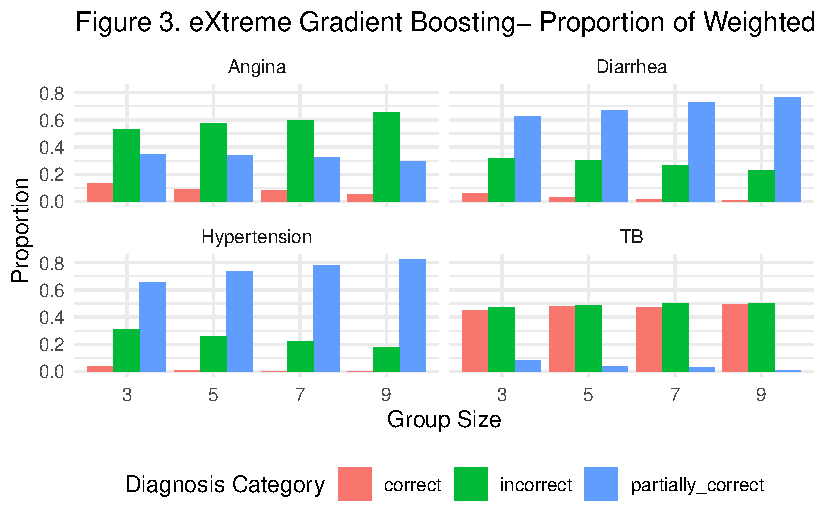
\includegraphics{simulation_files/figure-pdf/unnamed-chunk-5-1.pdf}




\end{document}
